% =====================================================================
%  ELAJ — manuscript for Nature Machine Intelligence
%
%  Atharva Waghmare
%
%  Build:  latexmk -pdf main.tex
%  or:     bash build.sh          (adds MacTeX to PATH first)
%
%  STRUCTURE MIRRORS Thesis/: main.tex + preamble.tex + sections/.
%
%  THE ORDER BELOW IS NATURE'S, NOT OURS. Nature journals run the
%  manuscript as: Abstract → Introduction (unheaded) → Results →
%  Discussion → Methods → Data and Code availability → References →
%  Acknowledgements → Author contributions → Competing interests →
%  figure legends → Extended Data → Supplementary Information.
%  Methods sits AFTER the references in the published article and is
%  NOT counted against the word limit, which is why it is being written
%  first and why it carries the detail.
%
%  NMI shape for an Article: main text about 3,500 words (abstract 200,
%  introduction ~750, results ~2,000, discussion ~1,000 at the outside),
%  up to eight display items, everything else in Extended Data.
%
%  WHAT IS WRITTEN AND WHAT IS NOT. Every section is \input so the whole
%  shape renders and the flow can be read off one PDF. Sections whose
%  prose is not written contain purposes in grey \note{} and nothing
%  else; the main text is deliberately held until the claim is settled.
% =====================================================================

\documentclass[11pt, a4paper]{article}

% =====================================================================
%  ELAJ — paper preamble
%
%  Adapted from Thesis/preamble.tex. What carries over and what does not:
%
%    KEPT   the palette, the \elaj macro, \todo/\note, booktabs, natbib,
%           the caption style, amsmath + bm
%    DROPPED two-column, extreport at 9pt, chapter machinery, the crest,
%           the float-fraction relaxations that two columns needed
%    ADDED  line numbers and 1.5 spacing for review, because this is a
%           drafting document that a supervisor and then a reviewer marks
%           up. Both come off for submission by flipping \draftmode.
%
%  Nature Machine Intelligence takes LaTeX at submission and typesets from
%  the accepted manuscript, so this file is for US, not for them. It is
%  deliberately plain: no journal class, nothing that would have to be
%  unpicked later.
% =====================================================================

\usepackage[a4paper, margin=2.5cm]{geometry}
\usepackage[british]{babel}
\usepackage[T1]{fontenc}
\usepackage{microtype}

% ---- Maths ----------------------------------------------------------
\usepackage{xspace}
\usepackage{amsmath}
\usepackage{amssymb}
\usepackage{bm}

% ---- Figures and tables ---------------------------------------------
\usepackage{graphicx}
\graphicspath{{figures/}}
\usepackage{booktabs}           % \toprule \midrule \bottomrule, never \hline
\usepackage{tabularx}           % Table S29: a value column that wraps at the text width
\usepackage{multirow}
\usepackage{array}
\usepackage{longtable}
\usepackage[font=small,labelfont=bf,justification=justified,
            singlelinecheck=false,skip=6pt]{caption}
\usepackage{subcaption}
\usepackage{float}

% ---- Colour ---------------------------------------------------------
\usepackage[dvipsnames]{xcolor}
% Matched to the project's figures so the document and the plots read as
% one system.
\definecolor{elajink}{HTML}{22223B}
\definecolor{elajteal}{HTML}{2A9D8F}
\definecolor{elajcoral}{HTML}{E76F51}
\definecolor{elajmuted}{HTML}{8D99AE}

% ---- References and links -------------------------------------------
\usepackage[
  colorlinks=true,
  linkcolor=elajink,
  citecolor=elajteal,
  urlcolor=elajteal,
  breaklinks=true,
]{hyperref}
\usepackage{url}
\usepackage[numbers,sort&compress]{natbib}
\bibliographystyle{unsrtnat}

% ---- Drafting apparatus ---------------------------------------------
% Set \draftmodetrue before submitting: it removes line numbers, the
% extra leading, and every \todo and \note in one switch.
\newif\ifdraftmode
\draftmodetrue

\usepackage{setspace}
\usepackage{lineno}
\ifdraftmode
  \onehalfspacing
  \linenumbers
  \renewcommand\linenumberfont{\normalfont\tiny\sffamily\color{elajmuted}}
\fi

% ---- Headings -------------------------------------------------------
\usepackage[explicit]{titlesec}
\titleformat{\section}{\normalfont\Large\bfseries\color{elajink}}{\thesection}{1em}{#1}
\titleformat{\subsection}{\normalfont\large\bfseries\color{elajink}}{\thesubsection}{1em}{#1}
\titleformat{\subsubsection}{\normalfont\normalsize\bfseries}{\thesubsubsection}{1em}{#1}
\titlespacing*{\section}{0pt}{2.2ex plus 1ex minus .2ex}{1.2ex plus .2ex}
\titlespacing*{\subsection}{0pt}{1.8ex plus 1ex minus .2ex}{0.9ex plus .2ex}

% ---- Project macros --------------------------------------------------
% Set in Comfortaa at 88% of the surrounding size, which cap-matches it to
% newtx. Loaded by family name rather than by package so nothing here can
% disturb the body font. See Thesis/preamble.tex for the measurement.
\makeatletter
\newcommand{\elaj}{{\fontfamily{comfortaa}%
  \fontsize{\the\dimexpr\f@size pt*88/100\relax}{\f@baselineskip}\selectfont
  \textls[150]{ELAJ}}\xspace}
\makeatother
\newcommand{\scrnaseq}{scRNA-seq\xspace}
\newcommand{\snrnaseq}{snRNA-seq\xspace}

% \color inside a group, NOT \textcolor: \textcolor is not \long, so a blank
% line inside a note would end the paragraph mid-argument and abort the build.
\newcommand{\todo}[1]{\ifdraftmode{\color{elajcoral}\small\bfseries[TODO: #1]}\fi}
\newcommand{\note}[1]{\ifdraftmode{\color{elajmuted}\small\itshape[#1]}\fi}
% Navigation between Methods subsections. Scaffolding for us, noise for a
% reader, and it used to survive \draftmodetrue because it was written
% as raw \textcolor rather than as a macro.
% DEAD since 9 November 2026: all nine \flow{} transitions were cut from
% Methods under the register review. Macro kept so the nine lines can be
% restored from git without touching the preamble.
\newcommand{\flow}[1]{\ifdraftmode\medskip\noindent%
  {\color{elajmuted}$\rightarrow$ \textit{#1}}\fi}


\title{\vspace{-2em}\elaj: Endometriosis Latent-space Analysis
through Joint-study modelling}
\author{%
  Atharva Waghmare\textsuperscript{1} \and Animesh Acharjee\textsuperscript{2,3,*}%
}
\date{%
  \normalsize
  \textsuperscript{1}Department of Computer Science, School of Engineering and
  Physical Sciences, University of Birmingham, B15 2TT.\\
  \textsuperscript{2}Department of Cancer and Genomic Sciences, School of
  Medical Sciences, College of Medicine and Health, University of Birmingham,
  B15 2TT.\\
  \textsuperscript{3}Centre for Health Data Research, University of
  Birmingham, B15 2TT, UK\\[4pt]
  \textsuperscript{*}Correspondence: Dr.\ Animesh Acharjee, Department of
  Cancer and Genomic Sciences, University of Birmingham, B15 2TT,
  Birmingham, UK. \texttt{a.acharjee@bham.ac.uk}%
}

\begin{document}

\maketitle

% =====================================================================
%  ABSTRACT — 150 words, unreferenced
% =====================================================================
% =====================================================================
% ABSTRACT. Third rewrite, 17 November 2026.
%
% AW's direction for this one: "What if we were to lead with the AI side
% instead of scale. Endometriosis is still the starting point. We add
% scale and some really innovative architecture. E3 is good but needs to
% be stated in a more understandable tone leading with the result. E4 is
% also a catchy result for a disease atlas." And: "'Claims no contributing
% cohort could test alone are settled' lines like these are not headline
% results."
%
% SO THE ORDER IS: endometriosis, then the architecture, then the scale,
% then what the atlas found. Scale is no longer the second beat; it
% arrives after the model has been described, as something the approach
% made affordable rather than as the claim itself.
%
% E3 NOW LEADS WITH THE RESULT AND NAMES THE GENES. The previous draft
% opened on the method ("Decoding that direction returns...") and said
% "four of its fifteen leading genes", which asks the reader to hold an
% abstraction. IBDex names its genes outright, DMBT1, DUOXA2, OLFM4,
% NOS2, CXCL1, and HLCA names SPP1+ macrophages, so naming them is in
% register for a disease atlas.
%
% E4 IS PROMOTED to its own sentence on AW's reading that four genes no
% prior endometriosis report contains is catchy for an atlas. It is the
% one claim here that is a discovery rather than a confirmation.
%
% THE META-SENTENCE IS GONE. "Claims no contributing cohort could test
% alone are settled" describes an activity, not a finding. What replaced
% it is the two findings themselves, with their donor counts.
%
% LENGTH. 236 words against NMI's 150 spec; the six NMI abstracts measure
% 147 to 203, median 183. AW, 17 November: "Feel free to go over, I can
% edit", and the standing rule is to seed complete rather than short. The
% cheapest cuts, in order: the frontier sentence (25 words, but it is
% result B1 at importance 10), the eight gene names (12 words), and the
% closing composition clause.
% =====================================================================

\begin{abstract}
\noindent
Endometriosis is diagnosed by surgery, so its biology has been studied one
small cohort at a time, and the field's reference atlas of the endometrium
spans 63 donors. Here we present \elaj, a single-cell disease atlas of
endometriosis in which biological structure built into the model replaces
pretraining scale. A conditional variational autoencoder reads each cell as
44 pathway groups rather than as fifteen thousand independent genes, and
returns sixteen interpretable dimensions. Two coefficients trace a frontier
along which donor identity is traded against retained biology, so every
result is reported from a named position on it. At 1{,}883{,}986 parameters
\elaj\ holds more menstrual-cycle signal at lower donor identity than nine
competing representations, foundation models over fifty times its size among
them. The atlas is built from 1{,}577{,}728 cells and 254 donors across
eleven studies, four times the donors of that reference atlas. Inside immune
cells it separates patients from controls on donors it never saw, at an AUC
of 0.708, and names the genes that carry the separation. Four of them,
SERPINB2, MMP27, LRRC15 and INHBA, were independently reported as raised in
patients by a cohort outside this corpus,
\textit{P}~=~4~\texttimes~10\textsuperscript{--7}; none of the genes at the
control end was. Four others, SIGLEC7, ADAMDEC1, ALPK2 and KCNH1, appear in
no prior endometriosis report. Across 194 donors cell composition does not
differ between patients and controls, and severity among patients is
recovered by neither the latent nor a cell count.
\end{abstract}


% =====================================================================
%  MAIN TEXT — skeleton only. Framing is deliberately deferred until
%  the biological results land; see docs/paper/OUTSTANDING.md.
% =====================================================================
% =====================================================================
% INTRODUCTION — NMI prints this with no heading of its own, running
% straight from the summary paragraph. The \section*{Introduction} below
% is scaffolding and comes out before submission; the Introduction is
% simply the text before the first Results subheading.
%
% REWRITTEN 17 November 2026 against INTRODUCTION_STRUCTURE.md, which was
% itself rewritten the same day. Two inputs govern it and the previous
% draft predated both: the one-line story settled 11 November, and the
% guide's five pointers from the 11 November group feedback (why scRNA,
% why endometriosis, why disease atlas, what other studies have shown,
% what foundation models can say at a single-disease level).
%
% SHAPE taken from IBDex's own Introduction, read in full: six
% paragraphs, every one closing on a short declarative that lands the
% point, one naming sentence, the questions as a tricolon mapping onto
% Results in order, and the contribution stated by contrast.
% =====================================================================

\section*{Introduction}

%[para about endo being hard]
Endometriosis is a disease where tissue resembling the inner lining of the
uterus grows outside it. It affects roughly 190 million people worldwide 
\citep{who2025endometriosis}. Despite the prevalence, it has no validated 
non-invasive test and a confirmed diagnosis requires laparoscopic surgery 
\citep{who2025endometriosis,bontempo2025diagnostic}, making large studies 
difficult. Scale is necessary for answering deeper questions about 
the disease and collation of data is necessary for achieving that scale.

%[para about single cell being a good idea]
Single-cell transcriptomics is the resolution at which that biology is
legible, because endometriosis is a change in what particular cells do
rather than in which organ is affected. Lesions carry transcriptional 
programmes of their own \citep{fonseca2023endometriosis,tan2022singlecell}. 
The unaffected endometrium of an affected person is already altered, so 
the disease is not confined to the lesion
\citep{duempelmann2026endometrium,shih2022menstrual}. Immune involvement
recurs across every study that looks for it
\citep{huang2023immune,chen2022adenomyosis}, and reference atlases now
describe the cell types of healthy endometrium across the cycle
\citep{mareckova2024heca}. Evidently, single cell transcriptomics has 
shown promising results in cohorts of tens of donors 
\citep{duempelmann2026endometrium,mareckova2024heca}.

%[para about foundation models not being enough]
A foundation model, built for representation of large amounts of 
biological information, is the wrong tool despite its scale.
Models pretrained across tens of millions of cells
\citep{cui2024scgpt,theodoris2023geneformer,hao2024scfoundation,heimberg2025scimilarity}
return one representation per corpus. Although they are a promising 
direction for multi-disease and multi-organ representations, their 
zero-shot behaviour is uneven \citep{kedzierska2025zeroshot}. 
Re-training or fine-tuning these models requires huge amounts of 
compute and does not provide any disease-specific guarantee. 
Additionally, endometriosis, being influenced by the menstrual 
cycle \citep{who2025endometriosis,garciaalonso2021endometrium}, is subject 
to the most drastic short term cyclicity in the human body 
\citep{salamonsen2021endometrial} that no model has been trained for.


%[para about disease atlases being a good idea]
To overcome the limitations of donor counts and avoid pitfalls of 
foundation models, other fields have looked to disease atlases. 
The Human Cell Atlas set out to map every cell type in the human body 
against one shared reference, and established that such a reference can 
outlive the studies that built it \citep{regev2017hca}. At organ scale, the 
Human Lung Cell Atlas integrated 49 datasets, 2.4 million cells from 486 
individuals, into a single reference spanning health and disease 
\citep{sikkema2023hlca}. In inflammatory bowel disease, scIBD then showed 
that published single-cell studies alone, with no new sequencing, are 
enough to assemble a disease-focused meta-atlas \citep{nie2023scibd}. 
While the individual results from these studies are promising, a recent
review of atlas construction concludes that no single protocol applies to
all disease atlases and thus a tailored approach based on the
pathophysiology of the disease is needed \citep{hrovatin2025atlases}. 

%[para about batch-phase confound]
In an effort to further our understanding of endometriosis, we collated every 
publicly available single-cell study of the disease in a corpus of 
1{,}577{,}728 cells from 254 donors across eleven studies. This corpus is 
not a sample of the field; it is the field. Interpreting this corpus is 
especially hard because of a structural issue. Every donor is biopsied once, 
so each contributes cells from a single point
in the menstrual cycle, so menstrual phase is constant within a donor. 
Structurally, this is the same as a batch-effect. A correction working on 
form alone would remove biological information as it removes batch-effects.
The field's guidance anticipates the general case and recommends coarsening 
the batch covariate, to dataset rather than to sample, wherever batches 
correspond to biological variables of interest \citep{hrovatin2025atlases}. 
However, its examples are all at dataset level and a phenotype constant within a 
subject due to single-biopsy donors is not among them. 


%[conclusion para]
We therefore built \elaj, a single-cell disease atlas of endometriosis 
that replaces foundation model-level scale with intelligently adapted 
inductive biases (Fig.~\ref{fig:model}a,b). \elaj\ is a 1{,}883{,}986 parameter transformer-based 
conditional variational autoencoder (CVAE) \citep{kingma2014auto, sohn2015learning} that groups a cell's genes 
into 44 biological pathway groups and compresses it into a 
sixteen-dimensional interpretable latent space.
Through \elaj\ we define a Pareto front on donor-blindness 
against retained cycle signal that we call the \elaj\ frontier. The 
model-family described in this paper dominates on the frontier and 
defines the parameters that control the position of a model on it. 
Through this disease atlas we evaluate the claims made by smaller 
datasets at a much larger scale, discover new genes associated with 
endometriosis, critically examine disease staging in endometriosis, 
and define an effective way of evaluating disease atlases. We evaluate 
our model through intensive ablation studies to define its limits.
% =====================================================================
% RESULTS — rewritten 13 November 2026 against RESULTS_STRUCTURE.md.
% The previous five-subsection version is in git history; nothing was
% carried over except the numbers, which are re-derived by
% audit_numbers.py on every build.
%
% REGISTER, measured against IBDex (the supervisor's own paper) rather
% than asserted. Targets, from its Results section:
%   mean sentence 17 words, median 16, longest 34
%   decimals per 100 words 5.5          (we were already at 5.6)
%   words of 9+ characters 23.1%        (we were at 11.5%, half)
% The gap is NOT number density. It is sentence length and vocabulary.
% Shorter sentences, heavier noun phrases, no term explained that an
% NMI reader already knows.
%
% STRUCTURE. Six subsections, headers stating the result per the
% supervisor's 9 November rule. R7 (how the field measures) moved to
% the Discussion on AW's 13 November ruling.
%
% No opening paragraph. NMI Articles go from the Results heading
% straight into the first subheading; the old "divided across 2 main
% categories" preamble was scaffolding and is cut.
% =====================================================================

\section*{Results}

% ---------------------------------------------------------------------
\subsection*{Batch effects and biology have a measurable trade-off}

Two training-time coefficients, the adversarial weight and the KL term,
position \elaj{} on a frontier rather than at an optimum. Across six arms
donor recovery spans 0.3975 to 0.5837 and cross-donor cycle agreement 0.5922
to 0.7346, varying monotonically together (Fig.~\ref{fig:knobs}a). What is
being removed is substantial: donor provenance is enriched 54.5-fold over
chance, 32.7\% of a cell's hundred nearest neighbours against 0.60\% expected
across 269 identifiers. Every donor contributed one biopsy, so menstrual
phase is donor-constant and no correction treating the donor as nuisance can
separate the two.

Adversarial pressure is not uniformly priced. Raising the weight from 7 to
168 reduces donor recovery from 0.5837 to 0.5188 at no measurable cost in
cycle agreement, 0.7337 against 0.7346. Raising it to 336 reverses both:
donor recovery returns to 0.5277 and cycle agreement falls to 0.7146. The
frontier has a knee, and the two arms reported throughout bracket it.
\elaj$_{B\,hi}$ holds cycle agreement at 0.7346 for donor recovery 0.5188;
\elaj$_{B\,lo}$ concedes cycle to 0.6033 and buys study mixing 0.6544 against
0.7613.

No competing representation reaches that frontier. Scored on the identical corpus,
\elaj$_{B\,hi}$ dominates all nine simultaneously on both axes. Donor
recovery is 0.5188 against their 0.5421 to 0.7892; cycle agreement is 0.7346
against their 0.4372 to 0.7303 (Fig.~\ref{fig:knobs}b). Four are pretrained
foundation models, and \elaj{} carries 1,883,986 parameters across sixteen
latent dimensions against scFoundation's 100 million across 3,072
(Fig.~\ref{fig:knobs}c). Across these ten, donor recovery predicts the
disease score ($\rho = +0.721$, $p = 0.019$). It does not predict cycle
agreement ($\rho = +0.176$, $p = 0.627$). The cycle advantage is therefore
not an artefact of retained identity.

% ---------------------------------------------------------------------
\subsection*{Sixteen dimensions carry cell identity and the menstrual
cycle}

Both labels are recovered cross-donor on all 1,577,728 cells with parameters
frozen, discarding same-donor neighbour pairs before scoring
(Methods, \emph{Whole-corpus embedding}). Cell family agreement reaches
0.9807 across 630,689 annotated cells from 118 donors ($p = 0.005$), and the
four compartments occupy contiguous, non-overlapping territory
(Fig.~\ref{fig:model}d). Cross-donor menstrual phase agreement reaches 0.6796
across 723,599 cells from 142 donors ($p = 0.005$). Phase was supplied to a
single linear classification head during training; cell family was supplied
to nothing, and emerges from reconstruction pressure and pathway grouping
alone.

Technical variation does not account for either. Under a best-of-sixteen
linear criterion, mitochondrial fraction, total counts and doublet score
reach 0.3396, 0.2514 and 0.1366. Serum progesterone reaches 0.4725 and
epithelial pseudotime 0.5801 (Supplementary Table~S1). That criterion
takes the strongest correlation available across sixteen dimensions, making
the technical values upper bounds. Biological covariates the model never
received still exceed every one of them.

% ---------------------------------------------------------------------
% R3 to R6 pending. See RESULTS_STRUCTURE.md.
% ---------------------------------------------------------------------

% =====================================================================
% DISCUSSION — rewritten 14 November 2026 against DISCUSSION_REGISTER.md,
% which was built by reading eight published Discussions in full: IBDex,
% scGPT, and six NMI papers (sources in Atharva Papers/NMI_register).
% The 6 November version is in git history.
%
% WHAT THAT READING CHANGED, and none of it was guessable:
%   1. NO MEASURED VALUES. Eight published Discussions quote six between
%      them; the old draft quoted 25. Data and cohort scale are quoted
%      freely; agreements, AUCs and rhos are not. One P value survives
%      here, as the hook for a mechanism, which is the one licensed use.
%   2. LENGTH TRACKS RESULTS. 30% across the six NMI papers, 44% in
%      IBDex. Results is 1,650 words, so the ceiling is ~840.
%   3. NO SUBHEADINGS, eight out of eight. The supervisor's four
%      sections are carried by a topic-sentence ladder instead: read the
%      first clause of each paragraph down the page.
%   4. CITATION-DENSE. Five of eight cite 12+ references. The old draft
%      cited one.
%   5. LIMITATIONS IN A SIGNPOSTED BLOCK near the end, never inside a
%      paragraph that is winning, and each one paired with its bound.
%
% The ladder, which is the structure:
%   1 what this establishes      2 foundation models    3 baselines
%   4 the field's instruments    5 single datasets      6 the clinic
%   7 limitations                8 future work          9 close
% =====================================================================

\section*{Discussion}

\elaj is a transformer-CVAE based disease atlas for endometriosis spanning 
eleven scRNA studies, 1{,}577{,}728 cells and 254 donors. Every donor was 
biopsied once, which created a confound between biology and batch effects 
\citep{hrovatin2025atlases}. \elaj's sixteen-dimensional latent space 
balances the trade-off by preserving endometriosis biology and limiting 
donor identity. Cell type clustering emerges in the latent without 
supervised training and the menstrual cycle is captured within relevant 
cell-type labels.

\elaj\ carries 1{,}883{,}986 parameters against scFoundation's 100 million, 
pretrained on over 50 million profiles \citep{hao2024scfoundation}. Four 
pretrained models conferred no advantage on this corpus over \elaj\
\citep{cui2024scgpt,theodoris2023geneformer,heimberg2025scimilarity,kedzierska2025zeroshot}.
scGPT's own authors note that its pretraining does not itself mitigate 
batch effects \citep{cui2024scgpt}. The architectural bet of replacing 
scale with inductive bias allowed \elaj to iterate for the best solution 
while keeping training cost low.

The \elaj frontier, defined on menstrual phase against donor or study identity,
is shaped by adversarial weight and information cost. While adversarial weight 
shifts the achievable trade-off until a critical value, giving worse results past 
it, the information cost slides the model along the trade-off. This shows 
that a single correction strength does not optimise the trade-off as 
assumed by simpler methods \citep{korsunsky2019harmony,lopez2018scvi,xu2021scanvi,hie2019scanorama}.

Cell composition does not differ between control and eutopic endometrium,
confirming at 194 donors a claim made in 60
\citep{duempelmann2026endometrium}. The claim that endometriosis abolishes
cyclical variation in immune composition failed at 112 and 101 donors against
the 13 that produced it \citep{huang2023immune}. The disease signal that does
survive lies inside immune cells, where decoding it returned macrophage-led
inflammation. Its leading genes overlap an independent cohort's upregulated
list at \textit{P}~=~3.95~\texttimes~10\textsuperscript{--7}
\citep{zhao2017transcriptome}, and two of them are absent from the resources
that index gene-disease associations \citep{cominelli2014mmp27}. Eleven
studies had converged on overlapping findings with no means of confirming one
another, because no two share donors or a cell vocabulary
\citep{mareckova2024heca}. Confirmation, contradiction, and external
replication are three functions a disease atlas is best suited to perform.

The rASRM staging does not hold in biological context. Whether a person has
endometriosis was recoverable from endometrium inside the uterus. Severity, 
a grouping derived from rASRM staging, was not legible without control samples.
A headcount of cell families did not separate severity either. Severity was 
only separable between control and disease cells indicating that rASRM staging 
does not align with biological signals.

Replacing the pathway grouping with random gene groups of identical sizes
degraded every biological axis, and disease status most of all. The inductive
bias is load-bearing rather than decorative. Removing the menstrual-phase head
left most of the cross-donor cycle agreement standing, which places that
signal in the architecture rather than in the one label the model was given.
Without that head the model also began overfitting from its first epoch, so
the supervision regularises as well as teaches.

The latent holds quantities nobody supplied it. Epithelial pseudotime and
serum progesterone are recovered more strongly than mitochondrial fraction,
library size or doublet score, so biology outranks technical variation across
the sixteen dimensions. Tissue of origin is the exception that confirms the
design: it is largely absent, because the decoder was handed it and the
encoder had no reason to keep it. Transferring cell-family labels through the
same space recovered them across studies accurately enough to carry the
composition tests above. Its one failure mode is instructive, since cell types
with no counterpart in the reference are absorbed silently, which bounds what
any latent space can be asked to annotate.

The negatives reported here are bounded by donor count rather than by biology,
because a permutation null's width is set by how many people contribute.
Surgical stage and severity are therefore claims that more donors could still
settle. Whether this architecture scales into a pretrained model is the
question these results raise and do not answer, since inductive bias and
corpus size are independent levers. Transfer beyond endometriosis rests on two
conditions rather than on the disease, scarce donors and severe batch
structure, which hold wherever diagnosis requires surgery. Other claims are
now limited by annotation rather than by scale. A less differentiated
epithelium has been reported in lesions from deconvoluted bulk and from
fourteen donors \citep{garciaalonso2021endometrium,tan2022singlecell}, and the
fifty-eight ectopic donors pooled here could test it directly once epithelial
subtypes are resolved. Because the model retrains in hours, each new cohort
can extend this reference instead of waiting on anyone to repeat a pretraining
run.

\elaj\ establishes a sixteen-dimensional reference for pooled endometrial
single-cell data. No competing representation reached its cross-donor cycle
agreement at a lower donor recovery, and none of the nine was better on both
axes at once. It prices donor removal against biology, recovers cell
identity and the cycle's compartment structure unsupervised, locates the
disease signal inside immune cells, and names genes the endometriosis
literature has not reported. Endometriosis
research has been held back by cohorts that cannot be read together. This is a
way to read them together.


% =====================================================================
%  METHODS — after the references in the published article, not counted
%  against the main-text limit. Written first.
% =====================================================================
% =====================================================================
% METHODS
%
% FLAT HEADINGS, which is what Nature asks for: "subdivided by short bold
% headings referring to methods used", each at most 40 characters. There
% is no nesting and no numbering in the submitted document. The group
% names below (THE CORPUS, INPUT REPRESENTATION, ...) are LaTeX comments
% only -- they are how we navigate the file, not structure in the paper.
%
% WHAT THE GREY NOTES ARE FOR. Each one states what its passage DOES --
% the question it answers, what it establishes, and what the next passage
% needs from it. Read end to end they are the spine of the section, so
% the flow can be judged before any of it is written. Provenance and
% word counts come last in each note, not first.
%
% ARROWS between groups name the question being handed forward.
%
% WORD BUDGET: ~3,500 target. Allocation: corpus 500 . input 500 .
% encoder 450 . latent 150 . decoder 700 . objective 450 .
% evaluation 550 . reporting 200.
%
% THE SINGLE-BIOPSY CONFOUND IS A THREAD, NOT A SUBSECTION. Stated in the
% Introduction, then called back wherever it forces a choice:
%   CALLBACK 1  donor-level splitting      (Study selection)
%   CALLBACK 2  the adversarial head       (Decoder)
%   CALLBACK 3  cross-donor evaluation     (Evaluation)
% =====================================================================

\section{Methods}

The methods section elaborates on the full \elaj pipeline. Starting from 
the data and its representation, we deconstruct all major architectural 
choices made in the model, and finally close with optimisation and 
efficiency measures. The results, ablation studies, and discussions are 
separated as this section only details the hypotheses for the choices made 
and not the outcome of those choices.

% =====================================================================
%  THE CORPUS  -- budget 500.
% =====================================================================

\subsection*{Study selection}

The corpus used in this project is a complete record of publicly 
available single-cell data for endometriosis. It combines eleven
single-cell and single-nucleus studies, 1{,}577{,}728 cells, 254 donors
and six anatomical sites.

The search followed the PRISMA 2020 reporting guideline. Five public
archives were queried automatically: OmicsDI, NCBI GEO, BioStudies and
ArrayExpress, CELLxGENE Discover, and the Human Cell Atlas Data Portal.
The term \texttt{endometriosis} was matched against title, description
and keyword fields over the fifteen years preceding the search. A sixth
archive, CNGBdb, was searched by hand.

A record had to satisfy three conditions to enter the corpus: the data
had to be of or contain single-cell RNA sequencing information; the
sample had to be biopsied human tissue; and the data had to be
relevant to endometriosis. The last constraint was left understated to
accommodate relevant studies that are not necessarily of endometriosis
patients. These studies were either of adenomyosis or of a normal 
physiological state. Adenomyosis was added because it is 
pathophysiologically related to endometriosis. Physiologically stable 
tissue was included to augment the control samples from other studies.

The corpus was de-duplicated by donor by referencing the paper published
for each dataset. Each donor was given a unique identifier. Tissue site
was mapped to UBERON terms and disease state to MONDO terms, so that a 
cell's origin is recorded in a standard form other datasets in the 
corpus can follow. No correction was applied to the expression values 
themselves.

Every study identifies the sample each cell came from, so every cell can
be traced to a donor. The corpus was split into training, validation and
test partitions targeting a 70/15/15 ratio, with every cell from a donor
placed entirely in one partition. Cells from one donor share a genotype,
a hormonal state, a handling protocol and in most cases a single biopsy,
so a cell-level split would place near-duplicates on both sides and
measure the model on cells it had effectively already seen. One study
pair deposits the same fifteen people under two sets of identifiers,
which the split could not detect; 17{,}873 held-out cells, 4.3\% of the
held-out set, therefore belong to a person who also appears under the
other study's identifier.


\todo{PRISMA figure. Its own display item, or panel (a) of a composite
Figure 1. Nature counts items not panels, so a composite costs nothing in
the item budget and only costs text length.}


\subsection*{Gene vocabulary}

The datasets in this corpus cover a heterogeneous set of genes. Gene
names are also not stable.

In an effort to standardise, every gene was resolved against the HGNC 
approved symbol set, with anything unresolved dropped and recorded against 
its study of origin. An alias pointing to two different approved symbols 
is ambiguous, and resolving it would mean guessing; all such aliases were 
dropped, removing 1{,}452 mappings.

With the names settled, the set of genes the model reads still has to be
chosen. The selection used here is derived from Reactome or Gene Ontology 
(GO) pathway groups.  A fixed vocabulary of 15{,}496 genes was taken as those 
annotated to at least one Reactome or GO pathway, on the reasoning that a
gene worth modelling is one known to participate in a biological process. 
This has added benefits apparent in the encoder later. Restricted to this 
vocabulary, the proportion of genes a pair of studies holds in common 
rises from 64–96\% to 87–98\%.

\medskip\noindent\textcolor{elajmuted}{$\rightarrow$ \textit{The corpus is
one object with a chosen vocabulary. How does a cell's counts over that
vocabulary become something a transformer can read?}}

% =====================================================================
%  INPUT REPRESENTATION  -- budget 500. NOT YET SEEDED.
% =====================================================================


\subsection*{Gene tokens}

A cell is passed to the model as a single datapoint: a sequence of
tokens, one per gene in the fixed vocabulary.

Each token is the sum of two parts. The first is a learned identity
embedding ($e_i$). This is a vector unique to a gene fixed for all cells. 
The objective of this embedding is to encode which gene we are referring 
to. It is a $d_{\text{token}}$ dimensional vector.

The second part encodes the magnitude of a gene's expression in a cell 
($c_i$). Gene expression in the raw input data is a number representing 
the occurrence of a gene in a given cell. This one-dimensional value is 
first library-normalised to a target sum of $10^4$ and log-transformed. 
The transformed value still needs to be projected to $d_{\text{token}}$
dimensions from one. To project it without collapsing all genes onto a 
single direction, we multiply the transformed value by a learnable 
square matrix of size $d_{\text{token}}$ ($A$) which is shared across 
all genes. The resultant scaled matrix ($c_i A$) is then multiplied by 
the gene identity vector to get a $d_{\text{token}}$ dimensional vector 
for gene expression. A gene token is therefore computed as:

\begin{equation}
\text{token}_i \;=\; e_i + c_i A e_i .
\label{eq:token}
\end{equation}

By using the gene identity vector in projecting gene expression values
we are able to avoid a trivial low-dimensional projection. The directions
of each gene expression value naturally differ because the gene identity
embedding is unique per gene. A trivial projection would collapse a
cell's entire expression profile onto a single line. Conversely, a 
per-gene learned expression embedding would also allow unique gene 
directions but introduce roughly 500{,}000 parameters to the model. 
Through this method we get away with a single matrix of roughly 1{,}000 
parameters and the identity and expression stay separable by construction.


\subsection*{Unmeasured genes and the sentinel}

Every entry in the corpus is marked as one of three things: a count, a 
measured zero, or not measured in this study. The third case is stored 
explicitly because zero is a value of expression and non-measured genes
cannot be assumed to have a value. None of the models compared in this paper 
carries an input state for a gene that was not assayed. While it can be 
argued that most entires in the raw counts are zero and thus it would 
make little difference to the model, we found it important to specify 
unmeasured genes to the model as a Did Not Sample (DNS) sentinel.

DNS sentinel is a distinct and reserved learned vector in place of a 
value embedding. Crucially, it does not impact the identity embedding of a 
gene. Which means it doesn't interfere with what a gene is, only how much it 
is measured. Unmeasured genes are also excluded from the reconstruction loss, 
since there is no observation to score a prediction against. This allows the 
model to develop a holistic and true understanding of a cell. More details 
about how much it affects the outcome are in the ablation studies section 
under results.


\subsection*{Pathway gene grouping}

Self-attention compares every token with every other token, so its cost
grows with the square of the sequence length. One token per gene over
15{,}496 genes is roughly 240 million pairs for a single cell. That is
where the parameters and the compute of most single-cell transformers go,
and it is why those models need to be trained on tens of millions of cells. 
This corpus has 1.58 million cells.

Previous models have either reduced the number of genes studied, compressed 
their input representation in a lossy manner, or just used a very large 
corpus. None of these are transferable to this model. Reducing the number 
of genes to the top two or three thousand most variable genes assumes that the 
genes that vary the most are the most relevant to the disease. We do not have 
any reason to believe this assumption holds for endometriosis. A lossy 
compression for input representation comes with similar assumptions.

Instead, we used the partitioning available through the Reactome and GO 
hierarchies and cut them into 44 groups. The hypothesis being that genes 
that work together biologically would have more interesting interactions 
and interactions between groups of genes would be more relevant than 
between individual genes belonging to different groups. Following this idea, 
attention is first run within each group and attention across groups is 
run afterwards. Consequently, attention work falls from 240 million pairs 
to 5.72 million, a reduction of 97.6\%, and no data-losing assumptions 
have been made.

Apart from parameter efficiency, gene grouping also increases the effective
subspace in which gene identity lives. Each group is processed independently, and
no cross-group gene interactions are attended to. The gene space is 
therefore block diagonal, one block per group, and the dimension actually 
available to represent a gene is the token width times the number of groups,
$32 \times 44 = 1{,}408$, rather than the token width alone. For
comparison, Gene2vec, which is the conventional off-the-shelf gene
embedding, uses 512 dimensions. Effectively, a 32-dimensional token here
is a slice of a gene space nearly three times wider than the standard one. The 
derivation is given in Supplementary Note 1.

The reason it is an effective space and the reason it is able to encode 
more information is the same: the block diagonal nature of the gene space 
matrix. Since a block diagonal matrix is a special case of a regular matrix, 
what each block contains is critical to expressing all genes. That is why 
the pathway grouping is relevant. Without that, we would be restricting the 
gene space to block diagonal and getting nothing in return. This is tested 
through an ablation study.


\medskip\noindent\textcolor{elajmuted}{$\rightarrow$ \textit{A cell is now
44 groups of tokens. What reads a group, and what does it hand on?}}

% =====================================================================
%  ENCODER  -- budget 450. Needs MORE than the thesis has: the funnel,
%  and how information is squeezed.
% =====================================================================

\subsection*{Group encoders}

Each group is read by its own transformer: two layers of multi-head
self-attention, four heads, operating on that group's input tokens at width
32. Within a group, attention models what any two genes are doing 
together in a cell. The summary of interactions inside each group is 
collected in a CLS token. What leaves the stage is essentially a summary of 
each group. 

Notably, this is the first and most stark compression in the model. A cell 
enters as 15{,}496 gene tokens and 44 summary tokens are created. A 350-fold 
reduction. Additionally, a learned CLS token reads the group through a single
query, and what it carries away is a weighted combination of what
that one query attended to. Which is to say, it is a lossy form of compression. A 
weighted average discards the shape of a distribution. To recover more 
information, \elaj{} concatenates eight order statistics computed over the 
group's gene tokens to the learned token. The mean, the standard deviation, 
the minimum, the three quartiles, the maximum, and the mean of the top four 
are the statistics appended. Each statistic becomes its own summary token 
rather than being folded into one wide vector, so the next stage sees them 
separately.

A group therefore hands on nine summary tokens instead of one, and the
hypothesis being made is explicit: a single learned query is a lossy
readout of a group of genes, and that order statistics recover part of
what the averaging throws away. Ablation C-4 removes the eight statistics
and keeps the learned token alone, taking what each group contributes from
288 numbers back to 32.

Now, a cell enters as 15{,}496 gene tokens and leaves this stage as 396 
summary tokens. A reduction of roughly 39-fold achieved without attending 
across the vocabulary and without dropping a gene.


\subsection*{Cell aggregation}

Up to this point the model has only looked at genes within different 
pathways independently. The second stage asks how the groups relate to one 
another.

The 396 group summaries are assembled into one sequence together with a
learnable cell summary token appended. The second stage of the encoder 
is a transformer with two layers, four heads, and width 64. The learned 
cell summary token is the first representation of the complete cell 
inside the model.

The purpose of this stage is to allow the model to understand interaction 
between the individually studied gene groups. The hypothesis being that 
at this stage the model learns biologically relevant cellular information 
from an analysis of known pathway groups.

The lossy compression objection raised one level down applies here too. 
Consequently, the same remedy is applied again: order statistics are 
computed over the group-token positions and merged with the cell token. 
The merge projects back to width 64 rather than widening the output.

A cell therefore leaves the encoder as a single vector of width 64,
narrowed from 15{,}496 gene tokens through 396 group summaries.


\medskip\noindent\textcolor{elajmuted}{$\rightarrow$ \textit{A cell is one
vector of width 64. What does the model keep when it is forced to describe
that cell in sixteen numbers?}}

% =====================================================================
%  THE LATENT  -- budget 150.
% =====================================================================

\subsection*{Latent space}

The latent is where the model's most compressed understanding of a cell 
is calculated. Everything before it works to populate it, and everything 
after it exists to check that what was put there is worth having. \elaj 
being a CVAE, its latent space is the main component of interpretation.

As with most CVAEs, \elaj compresses information into a Gaussian subspace. 
In practice, it is sixteen Gaussian distributions: sixteen means and 
sixteen variances. Compared to baselines, a sixteen dimensional subspace 
is tiny. We arrived at this experimentally rather than theoretically. More 
details are given in the results section.


\subsection*{Decoder conditioning}

Being a CVAE, \elaj passes metadata about a cell to the decoder. Only the 
deocder is conditioned in this model. Most importantly, the study a cell 
belongs to and the platform used for sequencing that cell, both of which 
help the model identify and isolate non-biological information, are 
passed as learned embeddings. Tissue is encoded into four levels: 
compartment, organ, tissue type, microsite. The combined metadata 
information is appended to the 64-dimensional projection of the 
16-dimensional latent space to give a combined 112-dimensional vector 
per cell to the decoder.

This whole exercise is done to remove batch effects and non-biologically 
relevant information from the latent. The exception is tissue details.
Tissue, referring to the site of biopsy, is provided to the decoder to 
remove the most obvious grouping of cells. Endometriosis is more than 
tissue identification. To uncover the biological signal beyond tissue, 
we remove the need to model tissue information.

Crucially, disease information is not given to the decoder. A decoder 
told which cells are diseased will not rely on the latent for the signal 
that separates a normal cell from a diseased one, which is 
counterproductive to understanding the through the latent space. Every 
disease result in this paper is therefore structure the model was never 
shown. However, one study is the sole source of both adenomyosis and 
myometrium in this corpus, so for those 49{,}606 cells the study 
embedding is also a disease indicator. Claims about adenomyosis are 
therefore selectively made.


\medskip\noindent\textcolor{elajmuted}{$\rightarrow$ \textit{The decoder
knows where the cell came from. Now it has to produce 15{,}496 numbers from
sixteen.}}

\subsection*{Reconstruction head}

The decoder of \elaj consists of 4 heads. The first, and the model’s 
primary objective, is reconstruction.

The reconstruction head turns the 112-dimensional context into one
predicted expression level for every gene the cell's study measures.
Between 13{,}144 and 15{,}056 genes are predicted, depending on the
study's DNS count. An output layer holding one row of weights per gene
would do this in 1{,}007{,}240 parameters, and would learn each gene's
response in isolation. \elaj scores genes against the cell instead, in
122{,}825 parameters.

\textbf{The design.} Each gene is given a 64-dimensional query vector,
derived from the 32-dimensional identity embedding the encoder uses as
input. The projections are unique per pathway group, making the 
weight and bias an accumulation of common information among genes in 
each group. This is what allows two genes in different groups to have 
similar identity embeddings without being confused for one another.

The cell context is read into two things: a 64-dimensional vector that 
scores against the gene query, and a scalar that scales the resulting 
profile. A gene's predicted log-expression is then given as:
\begin{equation*}
\log \mu_{ig} \;=\; \frac{(W_k c_i) \cdot q_g}{\sqrt{64}}
\;\big(\mathbf{w}^\top W_v c_i\big) \;+\; b ,
\end{equation*}
where $q_g$ is gene $g$'s query, $c_i$ is cell $i$'s context, and $W_k$,
$W_v$, $\mathbf{w}$, and $b$ are learned. $(\mathbf{w}^\top W_v c_i)$ is a
scalar value. Since there is no per-gene value vector of the kind a regular
attention layer would have, this is a bilinear scoring layer, closest in
form to scGPT's masked-value-prediction head.

\textbf{No per-gene baseline.} Every term above is multiplied by something
belonging to the cell, so no parameter gives a gene a constant expression
level. Most count decoders end in a per-gene linear layer whose bias
supplies exactly that, making the average expression profile free; here it
has to be delivered through the latent or the covariates.

\textbf{From scores to counts.} Capture depth varies by an order of 
magnitude across this corpus. So instead of asking the model to recreate 
the exact counts, we pose a simpler problem: predict how much each gene 
contributes to the total count of the cell. The model gets library size, 
total count of genes in a cell, as input for this task.

\textbf{The likelihood and the target.} The model predicts the mean 
count of each gene, and the observed counts are scored against a negative 
binomial with one dispersion learned per gene. The loss is the mean 
negative log-likelihood over all cells and all measured genes, so every 
reconstruction figure in this paper is in nats per gene. Genes hidden 
from the encoder during training are still demanded of the decoder, 
which makes this masked autoencoding.


\medskip\noindent\textcolor{elajmuted}{$\rightarrow$ \textit{A reconstruction
exists. What stops it being produced WITHOUT the latent?}}

\subsection*{Adversarial study removal head}

The second head of the decoder is an adversarial network designed to 
actively remove batch information from the latent. The network is trained to 
predict the study that a cell came from given the latent. It is given the 
latent means rather than sampling from the gaussian space. This 
removes variational noise that the adversarial head does not need to model. 
To make it an adversarial network, during backpropagation the gradient is 
reversed before reaching the latent, making discriminator performance a 
pressure against batch information.

Two weights govern this. One is the share of total loss attributed to the 
discriminator which governs how much the model optimises for discrimination. 
The other is the scaling factor of the reversed gradient. This determines 
how much the discriminator affects the encoder. It is the second that 
traces the frontier reported in this paper. 

As with any adversarial network, the discriminator's capacity is a sensitive 
hyperparameter. A strong discriminator prevents the model from learning 
anything while a weaker one is easily fooled by the encoder. The failure 
mode of a weaker discriminator is described in results. \elaj uses a 
discriminator with three linear layers of width 256, with a leaky rectifier, no
dropout, and layer normalisation after each layer.


\medskip\noindent\textcolor{elajmuted}{$\rightarrow$ \textit{One term pushes
structure OUT of the latent. The next two decide what stays in.}}

\subsection*{Elastic cell similarity head}

The third head of the decoder is a selective pressure head adapted from 
scGPT. Notably, this head acts pairwise on the cell embeddings within a 
batch and not against one cell. Every pair of cells is checked against a 
cosine similarity threshold of 0.8. Pairs falling below the threshold are 
pushed away from each other while cells that clear the threshold are pulled 
closer together and pairs at or below zero cosine are left untouched. 

In practice this acts as a sharpening term and its purpose is to make a 
collapsed latent expensive. A single undifferentiated cloud is as 
uninformative as clear study-sectioned clouds. This head stretches 
dissimilar cells in a batch while simultaneously pushing similar cells 
together. Crucially, every pair is drawn from one study because a batch is 
composed of one study by construction. A cross-study pair of the same cell 
type with a low cosine because of batch effects would be driven further 
apart instead of closer. That puts unnecessary pressure on the adversarial 
head. Confined to one study the term can sharpen within-study structure, 
which helps gather biologically similar cells together.


\medskip\noindent\textcolor{elajmuted}{$\rightarrow$ \textit{Both terms so
far shape the latent without being told anything. One term is told.}}

\subsection*{Menstrual-phase head}

The fourth head is the only head other than reconstruction that introduces
new information in the model rather than moulding existing information. 
Cycle phase is among the largest sources of biological variation in
endometrium. The menstrual phase head is a linear classifier 
that reads the Gaussian latent means and predicts the cell's 
menstrual-cycle phase.

The reconstruction head has no pressure to isolate menstrual cycle. Each 
donor contributes a single biopsy in this corpus which is a data confound 
that needs to be taken into consideration. That relates directly to the
adversarial head as it acts against menstrual cycle information simply 
because it has the same geometric form as a study effect. The menstrual 
phase head gives that trade-off a second side, so moving the adversarial 
strength traces a frontier rather than erasing both at once.

However, a head with hidden layers would learn how to separate the latent
nonlinearly which doesn't necessarily make the latent more informative. 
Instead \elaj uses a single linear map that puts the separation pressure 
directly on the latent, creating a more interpretable subspace. 

Notably, \elaj is only semi-supervised on menstrual phase because 
512{,}101 of 1{,}161{,}472 training cells have menstrual phase metadata.
Unlabelled cells are not penalised. The effects of this head are quantified
through ablation studies described in results.

Menstrual phase is the only label the model is given. Cell type, disease 
status, stage and grade have no head in any configuration reported here, 
so every result on those is unsupervised.


\medskip\noindent\textcolor{elajmuted}{$\rightarrow$ \textit{Five terms
exist. What does the sum look like?}}

\subsection*{Composite objective}

The four heads are trained together through one loss value. 
Reconstruction acts over all genes with weight 1 while every other 
term is weighted against it as:
\begin{equation*}
\mathcal{L} \;=\; \mathcal{L}_{\text{nb}}
\;+\; \frac{1}{G}\Big[\,
\beta(t)\, w_{\text{kl}}\, \mathcal{L}_{\text{kl}}
\;+\; w_{\text{ecs}}\, \mathcal{L}_{\text{ecs}}
\;+\; w_{\text{dab}}\, \mathcal{L}_{\text{dab}}
\;+\; w_{\text{cls}}\, \mathcal{L}_{\text{cls}}
\,\Big] ,
\end{equation*}
with $w_{\text{kl}}$ 1, $w_{\text{ecs}}$ 50, $w_{\text{dab}}$ 0.5 and
$w_{\text{cls}}$ 40. Reconstruction is a mean over genes while the four
bracketed terms are per-cell quantities, so each is divided by the number of 
genes that batch's study measured ($G$).

The price on the latent is the usual one: the Kullback--Leibler divergence
between each cell's posterior and a unit Gaussian, summed over the sixteen
dimensions and averaged over cells. $\beta(t)$ ramps it linearly from zero
over the first 5\% of training steps, reaching 0.5, because until
reconstruction is established the latent holds nothing worth paying for and
a full price collapses it first. $w_{\text{kl}}$ is the second of the
paper's two knobs: at a fixed adversarial strength it moves the model along
the frontier rather than displacing the frontier itself.
information cost and is described next.

$\lambda_{\text{dab}}$ is absent from this sum, which is deliberate. It
scales the gradient as it is reversed on the way to the encoder, so it
governs how much of the adversarial loss the latent feels while leaving the
discriminator's own training untouched. That is the knob which traces the
frontier, and it is set to 168 in the reported arm. Only the first two 
terms are the model's own objective. Checkpoint selection and early 
stopping read reconstruction alone.


\subsection*{Cross-donor agreement}

In this corpus, every donor was biopsied only once. This has repercussions in
how the model performance should be measured on this corpus. Because a donor
contributes a single sample, that donor has exactly one menstrual phase, one
disease status, one stage and one grade, and every cell drawn from them
inherits those values unchanged. Each of these labels is therefore a property
of the donor rather than of the cell. Cell type is the only exception: it
varies within a single biopsy.

The obvious way to ask whether a latent carries a label is to check whether
cells agree with their neighbours: take each cell's nearest neighbours in the
latent and measure how often they share its label. On this corpus that test
cannot be trusted, and the reason is the paragraph above. If a label belongs
to the donor, then asking whether a cell's neighbours share its label is
asking whether they come from donors carrying that label, and a cell's own
donor carries it by definition. Every neighbour drawn from the same donor is
an automatic match, scored whether or not the latent encodes anything about
the label at all.

Plain agreement therefore rests on a floor set by how many of a cell's
neighbours come from its own donor, and on this corpus that floor is high.
Among the hundred nearest neighbours of a labelled cell, between a quarter
and three-fifths belong to the same donor depending on the label: 37\% for
menstrual phase, 29\% for disease status, 61\% for stage. A latent carrying
no donor information at all would give the chance rate, the probability that
two cells drawn at random share a donor, which is between 0.6\% and 3.1\%
here. Same-donor neighbours are thus twenty to fifty times over-represented,
and because each is an automatic match that enrichment passes straight into
the score: of the agreement a plain measurement reports, between 44\% and
71\% is the free same-donor part.

Worse, it is a floor the model can raise. A model that learns to recognise
donors increases the share of its own donor among each cell's neighbours and
improves its own score, so ranking models by plain agreement partly ranks
them by how well they memorised the donor, the opposite of what this
paper is measuring.

\elaj\ is measured with the same-donor neighbours removed. For each label,
the hundred nearest neighbours of every labelled cell are found in the
sixteen-dimensional latent and collected into a donor-by-donor matrix: entry
$(d, d')$ counts how many neighbours of donor $d$'s cells belong to donor
$d'$. The diagonal is then discarded (that discarding
is what cross-donor means), and agreement is the share of the remaining neighbour relations
that join two donors carrying the same label. Chance is the probability that
two such relations drawn at random would share a label, $\sum_j p_j^2$ over
the label's shares across donors, and agreement is reported as excess over
it, $(a - c)/(1 - c)$, so labels with different numbers of levels are
comparable.

The null is obtained by reassigning labels to donors. Two hundred random
permutations of the donor-to-label map are scored through the same
expression, which asks what agreement this latent would produce if the same
labels had been dealt to different donors, the appropriate null for a
quantity constant within a donor. The reported $p$ is the share of
permutations reaching the observed agreement, counted as
$(1 + \#\{\text{null} \geq \text{observed}\}) / (1 + 200)$.

That construction puts a floor under $p$, and the floor matters for reading
this paper's negative results. With two hundred permutations the smallest
attainable value is $1/201$, and more restrictively the number of distinct
permutations is set by how many donors carry the label at all. Where a label
reaches only a handful of donors, no arrangement of them can produce a small
$p$, so a result that is not significant means the test could not detect an
effect of any size rather than that no effect exists. Disease stage and
endometriosis grade reach 58 and 60 donors respectively, against 269 for
disease status, and are reported as undetectable rather than absent.

Because the labels are constant within donors, the matrix is a sufficient
statistic: agreement and its null are arithmetic on a table of integers with
at most one row per donor, and the neighbour search that produced it is the
only step needing the whole corpus in memory. Any later regrouping of a label
is recomputed from the stored matrix without re-embedding a cell.

The construction is a permutation test of assortativity on a fixed graph.
The statistic is the share of edges joining same-label nodes, which is the
enumerative mixing coefficient of \citet{newman2003mixing} computed on a
donor graph rather than its usual node graph; significance by permuting group
identities against an unchanged proximity structure is the procedure of
\citet{anderson2001permanova}; and permuting at the level of the donor rather
than the cell is what \citet{squair2021confronting} prescribe, since donors
and not cells are the independent replicates in a multi-donor single-cell
study.

\note{THIS SUBSECTION IS NOT REVIEWED. AW, 2 November 2026. Everything
below was established by reading
\texttt{endo\_model/evaluation/sufficient\_stats.py} on 2 November and is
recorded here because the prose depends on it and because one error had
already propagated out of it. The same material is in
\texttt{axw1008/docs/paper/CROSS\_DONOR\_ESTIMATOR.md}.
\\
\\\textbf{WHAT THE TEST IS, IN ITS OWN VARIABLES.}
\\\quad $\bullet$ \texttt{matrix} is donor $\times$ donor. Entry $(d,d')$
counts how many of donor $d$'s cells' hundred nearest neighbours belong to
donor $d'$.
\\\quad $\bullet$ \texttt{np.fill\_diagonal(matrix, 0.0)} deletes the
same-donor relations. \textbf{The off-diagonal is the cross-donor part};
zeroing the diagonal is what makes it so. An earlier draft of this note had
that backwards.
\\\quad $\bullet$ \texttt{lab} holds \emph{one label per donor}, which is
only legitimate because the label is donor-constant.
\\\quad $\bullet$ \texttt{agree(assignment)} is
\texttt{(m * same).sum() / total}: of every cross-donor neighbour relation,
the share joining two donors with the same label.
\\\quad $\bullet$ \texttt{observed = agree(lab)}.
\\
\\\textbf{THE HYPOTHESES.} $H_0$: the latent's donor-level geometry is
unrelated to the label, so the observed agreement is what any assignment of
these labels to these donors would give. $H_1$: donors sharing a label sit
closer, so their cells fall in each other's neighbourhoods more often.
\\
\\\textbf{WHAT IS PERMUTED, AND WHAT IS NOT.} The embedding and the
neighbour graph are computed once and never change. Cells do not move and
donor membership does not change. Only \texttt{lab} is permuted: the same
labels are dealt to the same donors in a different order. The donor is the
exchangeable unit because the label is constant within one, so nothing below
donor level can carry information about it; permuting cell labels would break
that constancy and build a null so weak that everything would pass.
\\
\\\textbf{\texttt{chance} AND THE NULL ARE NOT THE SAME THING, AND ONLY ONE
IS CALIBRATED.} \texttt{chance} is $\sum_j p_j^2$ over the label's shares
\emph{across donors}, weighting every donor equally. But \texttt{observed}
weights each donor pair by the neighbour relations between them, so large and
tightly-clustered donors dominate it. The two are computed under different
weightings, which makes \texttt{excess} $= (a-c)/(1-c)$ a descriptive effect
size with an approximate correction rather than a calibrated one.
\textbf{The permutation $p$ is the inferential statistic}, because it
recomputes under the same weighting.
\\
\\\textcolor{elajcoral}{\textbf{LOOPHOLES, WORST FIRST. These belong in the
Discussion's limitations, not here.}
\\1. \textbf{\texttt{excess} is not comparable across labels, which was the
stated purpose of normalising it.} The null's own 95th percentile, carried in
the benchmark \texttt{note} column, tracks donor count: 0.06 at 34 donors
(cell family), 0.18 at 36 (phase), 0.12 at 18 (grade), \textbf{0.42 at 16}
(stage). Reassigning sixteen donors' labels at random reaches 0.42, so
reading 0.1313 and 0.7346 on one scale is wrong.
\\2. \textbf{$p$ is one-sided} --- \texttt{(null >= observed).sum()}. It can
never establish a significantly \emph{negative} value, so grade's
$-$0.0414 is ``not positive'', never ``negative''.
\\3. \textbf{For a label spanning several studies the permutation is too
permissive.} Disease status covers 269 donors across eleven studies and some
cohorts are entirely cases, so permuting across all of them destroys the
label--study association and the null never sees the study structure partly
producing the observed agreement. This is visible in our own numbers: pooled
disease status is significant at $p=0.005$, and inside each cohort, where the
permutation is necessarily within-study, nothing is
($p=0.3433$, $0.0697$, $1.000$). Stage and grade are unaffected because every
labelled donor for each sits in one cohort.
\\4. \textbf{The permutation is unstratified by donor size}, so one draw can
hand a label to donors carrying very different adjacency mass. A size-matched
permutation would give a tighter null.
\\5. $k=100$ is a free choice the statistic depends on, with no sensitivity
analysis.
\\6. $p$ floors at $1/201$, so 0.005 means ``nothing in two hundred beat
it'', not a measured small probability.}
\\
\\\textcolor{elajcoral}{\textbf{A CLAIM IN THE PROSE ABOVE IS WRONG AND
NEEDS CUTTING ON REVIEW.} ``the number of distinct permutations is set by how
many donors carry the label at all'' is not the binding constraint at 16 to
60 donors, where the number of distinct assignments is astronomical. What
binds is the \emph{width} of the null, which is loophole 1. The p-floor
argument should be made that way instead, and it is the stronger version.}}





\subsection*{Donor and study recovery}
\note{PURPOSE: define the two costs, so the frontier has both its axes
before it is plotted. These are the quantities a good model should fail
at.\\
HANDS ON: both axes exist. What does the latent's shape look like under
them?\\
SOURCE: Thesis 05 §Study mixing.}



\subsection*{Whole-corpus embedding}
\note{PURPOSE: licence the paper's discovery half. Once the model is
fixed, nothing is being selected, and the metadata read below was never
an input --- so there is nothing a held-out split protects against for
these labels, and all 1{,}577{,}728 cells can be embedded and read
together. Phase is the exception, governed by the head. Also the region
procedure: every cell takes the cell family of its 25 nearest LABELLED
neighbours searched in the sixteen dimensions, not in the UMAP, because a
bounding box assumes each family occupies one convex patch and immune
cells do not.\\
SOURCE: new.}

\medskip\noindent\textcolor{elajmuted}{$\rightarrow$ \textit{Everything
measurable has been measured. What has to be declared?}}

\subsection*{Optimisation}
\note{PURPOSE: how a run is executed, kept short. AdamW, $10^{-3}$, batch
256, bf16, cosine over a 20-epoch horizon chosen for its SHAPE rather
than its length --- the horizon sets how long the learning rate stays
high, and early stopping is what ends a run. Per-study batch construction
and domain-specific normalisation are two sentences here rather than
headings of their own, per your note that most training-procedure
material is statements belonging inside other passages.\\
HANDS ON: runs finish. Which checkpoint is the model?\\
SOURCE: Thesis §Configuration (72). Hyperparameter detail $\rightarrow$
Supplementary.}

% =====================================================================
%  REPORTING  -- budget 200. NOT YET SEEDED.
% =====================================================================



\subsection*{Use of large language models}

This project used generative artificial intelligence. None of the
architectural, experimental, curative, scientific, interpretive or
directional decisions were made by it. In descending order of usage, Claude
Opus 5, Claude Sonnet 4.8 and Claude Sonnet 4.5 were used, accessed
primarily through Claude Code, and the tasks fall into three groups. The
first is code writing. The system was given the project plan, the code flow
and the programmatic architecture, and was required to document every module
it wrote; the code was then reviewed manually against that documentation.
The second is testing. Unit, smoke and pre-flight tests were a standing
requirement of every module from the outset, which produced over 1{,}450 tests
across 115 files and made debugging and maintenance a part of writing rather
than a separate stage. The third is proofreading, including a search for
logical gaps in this manuscript and in the analysis that precedes it. Every
number reported here is additionally checked by two independent auditing
scripts that trace it to a named file, and a manuscript cannot be built with
an unsourced value in it.

\subsection*{Data availability}

This study analysed previously published data and generated no new primary
data. All datasets are publicly available: Gene Expression Omnibus
accessions GSE266265, GSE247695, GSE214411, GSE218044, GSE213216, GSE203191
and GSE179640; ArrayExpress accession E-MTAB-14039; and CellxGene Discover
collections \texttt{9ddea8d9} and \texttt{968885c5}.
CNGBdb accession CNP0006183 (li et al.).


\subsection*{Code availability}

All code for data preparation, model training and evaluation is available at
\textcolor{elajcoral}{[repository URL]} under an
\textcolor{elajcoral}{[MIT]} licence.



% =====================================================================
%  MANDATORY STATEMENTS, ACKNOWLEDGEMENTS, DISPLAY ITEMS
% =====================================================================
% =====================================================================
% BACK MATTER — Nature's mandatory statements, in Nature's order. These
% are short, they are checked by the editorial office before a paper
% goes to review, and a missing one delays the submission, so the
% headers exist from the start even though the text does not.
%
% ORDER IS NOT OURS TO CHOOSE. Nature journals run:
%   Data availability  →  Code availability  →  References  →
%   Acknowledgements  →  Author contributions  →  Competing interests  →
%   Figure legends  →  Extended Data  →  Supplementary Information
% Data and Code availability sit at the END OF METHODS, before the
% reference list; everything from Acknowledgements on follows it.
% =====================================================================

% ---------------------------------------------------------------------
% ---------------------------------------------------------------------
%  DATA AVAILABILITY and CODE AVAILABILITY were stubs here and are now
%  WRITTEN, in sections/04-methods.tex. Nature places both at the end
%  of Methods, before the reference list, which is where they are. The
%  stubs are removed rather than left as a second copy for the two to
%  drift apart.
%
%  One correction the old stub carried and got wrong: it said
%  GSE213216's citation ``must name the Nature Genetics original''. The
%  journal is not verified anywhere in the project. What IS established
%  (OUTSTANDING.md) is that the PDF on file is Pei et al. 2023, a
%  RE-ANALYSIS that used the accession rather than the original
%  submission. Find the original before naming a journal.
% ---------------------------------------------------------------------

% ---------------------------------------------------------------------
%  After the reference list
% ---------------------------------------------------------------------
\subsection*{Acknowledgements}

The authors acknowledge the use of BlueBEAR, the University of Birmingham's
high performance computing service, and of the associated BEAR Research Data
Store. \textcolor{elajcoral}{[Supervision, funding and grant numbers to be
added. BlueBEAR's own form of words to replace the sentence above.]}

\subsection*{Author contributions}

A.W. designed and implemented the model, ran the experiments, performed the
analysis and wrote the manuscript. A.A. supervised the project throughout,
and advised on its direction, design and interpretation. Both authors read
and approved the manuscript.

\subsection*{Competing interests}

The authors declare no competing interests.

\todo{Nature also requires a Reporting Summary at submission — a
separate form, not part of this document. Noting it here so it is not
discovered on the day.}

% =====================================================================
% DISPLAY ITEMS — six for the main text, and the reason panels are the
% cheapest real estate in this paper.
%
% NMI, Content Types, Article: "Main text — up to 3,500 words,
% EXCLUDING abstract, Methods, references AND FIGURE LEGENDS."
% "Display items — up to 6 items (figures and/or tables)."
%
% Nature, Formatting guide: "Each figure legend should begin with a
% brief title for the whole figure and continue with a short description
% of each panel... Legends should be fewer than 300 words each." And a
% composite figure with several panels "usually needs to take about half
% a page, equivalent to about 600 words, in order for all the elements
% to be visible".
%
% THE STRATEGIC CONSEQUENCE. Legends do not count against the 3,500, so
% six figures at up to 300 words of legend each is up to 1,800 words of
% free exposition. A finding that lives in a panel and its legend costs
% ZERO main-text words; the same finding enumerated in prose costs
% around 125. We have roughly twenty findings and 2,000 words of
% Results, so the figures are not illustrations of the prose — they
% carry findings the prose then points at.
%
% What a half-page composite costs is PAGE space, which is the editor's
% layout problem rather than our word budget. So: every main figure is a
% composite, panels are used generously, and legends are written to the
% 300-word limit rather than kept brief.
%
% Each figure must be regenerable by one command from a committed
% script — reproducibility item R5, cheaper to honour while building.
% =====================================================================

\section*{Display items}

\note{SIX MAIN FIGURES, mapped against RESULTS\_STRUCTURE.md's finding
labels so nothing is orphaned and nothing is carried twice. Status is
whether the panel exists today.}

\subsection*{Figure 1 --- \elaj\ as a model, and the main findings}
\note{ORDER SETTLED BY AW: 1 \elaj\ as a model and the main findings; 2 the
frontier; 3 both latents; 4 nine UMAPs; 5 the ablations. FIVE items, not six.
\\Recovered from the transcripts rather than re-invented: the architecture as
one long wide butterfly panel across the top, the frontier at \textbf{b} and
\textbf{c}, three UMAPs along the bottom.
\\PANELS SETTLED 7 November 2026, AW. The PRISMA diagram becomes
\textbf{d}, replacing the spider chart, and \textbf{b} and \textbf{d} swap
so the corpus is assembled before the frontier is drawn. Nature counts items
rather than panels, so PRISMA costs nothing against the five-item budget and
Methods no longer carries it as an open question. Order is therefore the
architecture across the top, PRISMA, the two frontier scatters, then the
UMAPs.
\\NOT RENDERED FINAL. Known defects: whitespace, clipped boxes, a chance
line drawn at 0.370 which is the double-counting error now corrected
everywhere else, and two separate Pareto fronts where Figure 2 draws one. The
frontier panels also overlap Figure 2 and that overlap has not been resolved.
\\UNBLOCKED: the four remaining arms' full-split mixing landed on
6 November, so every frontier point now exists.}

\begin{figure}[p]\centering
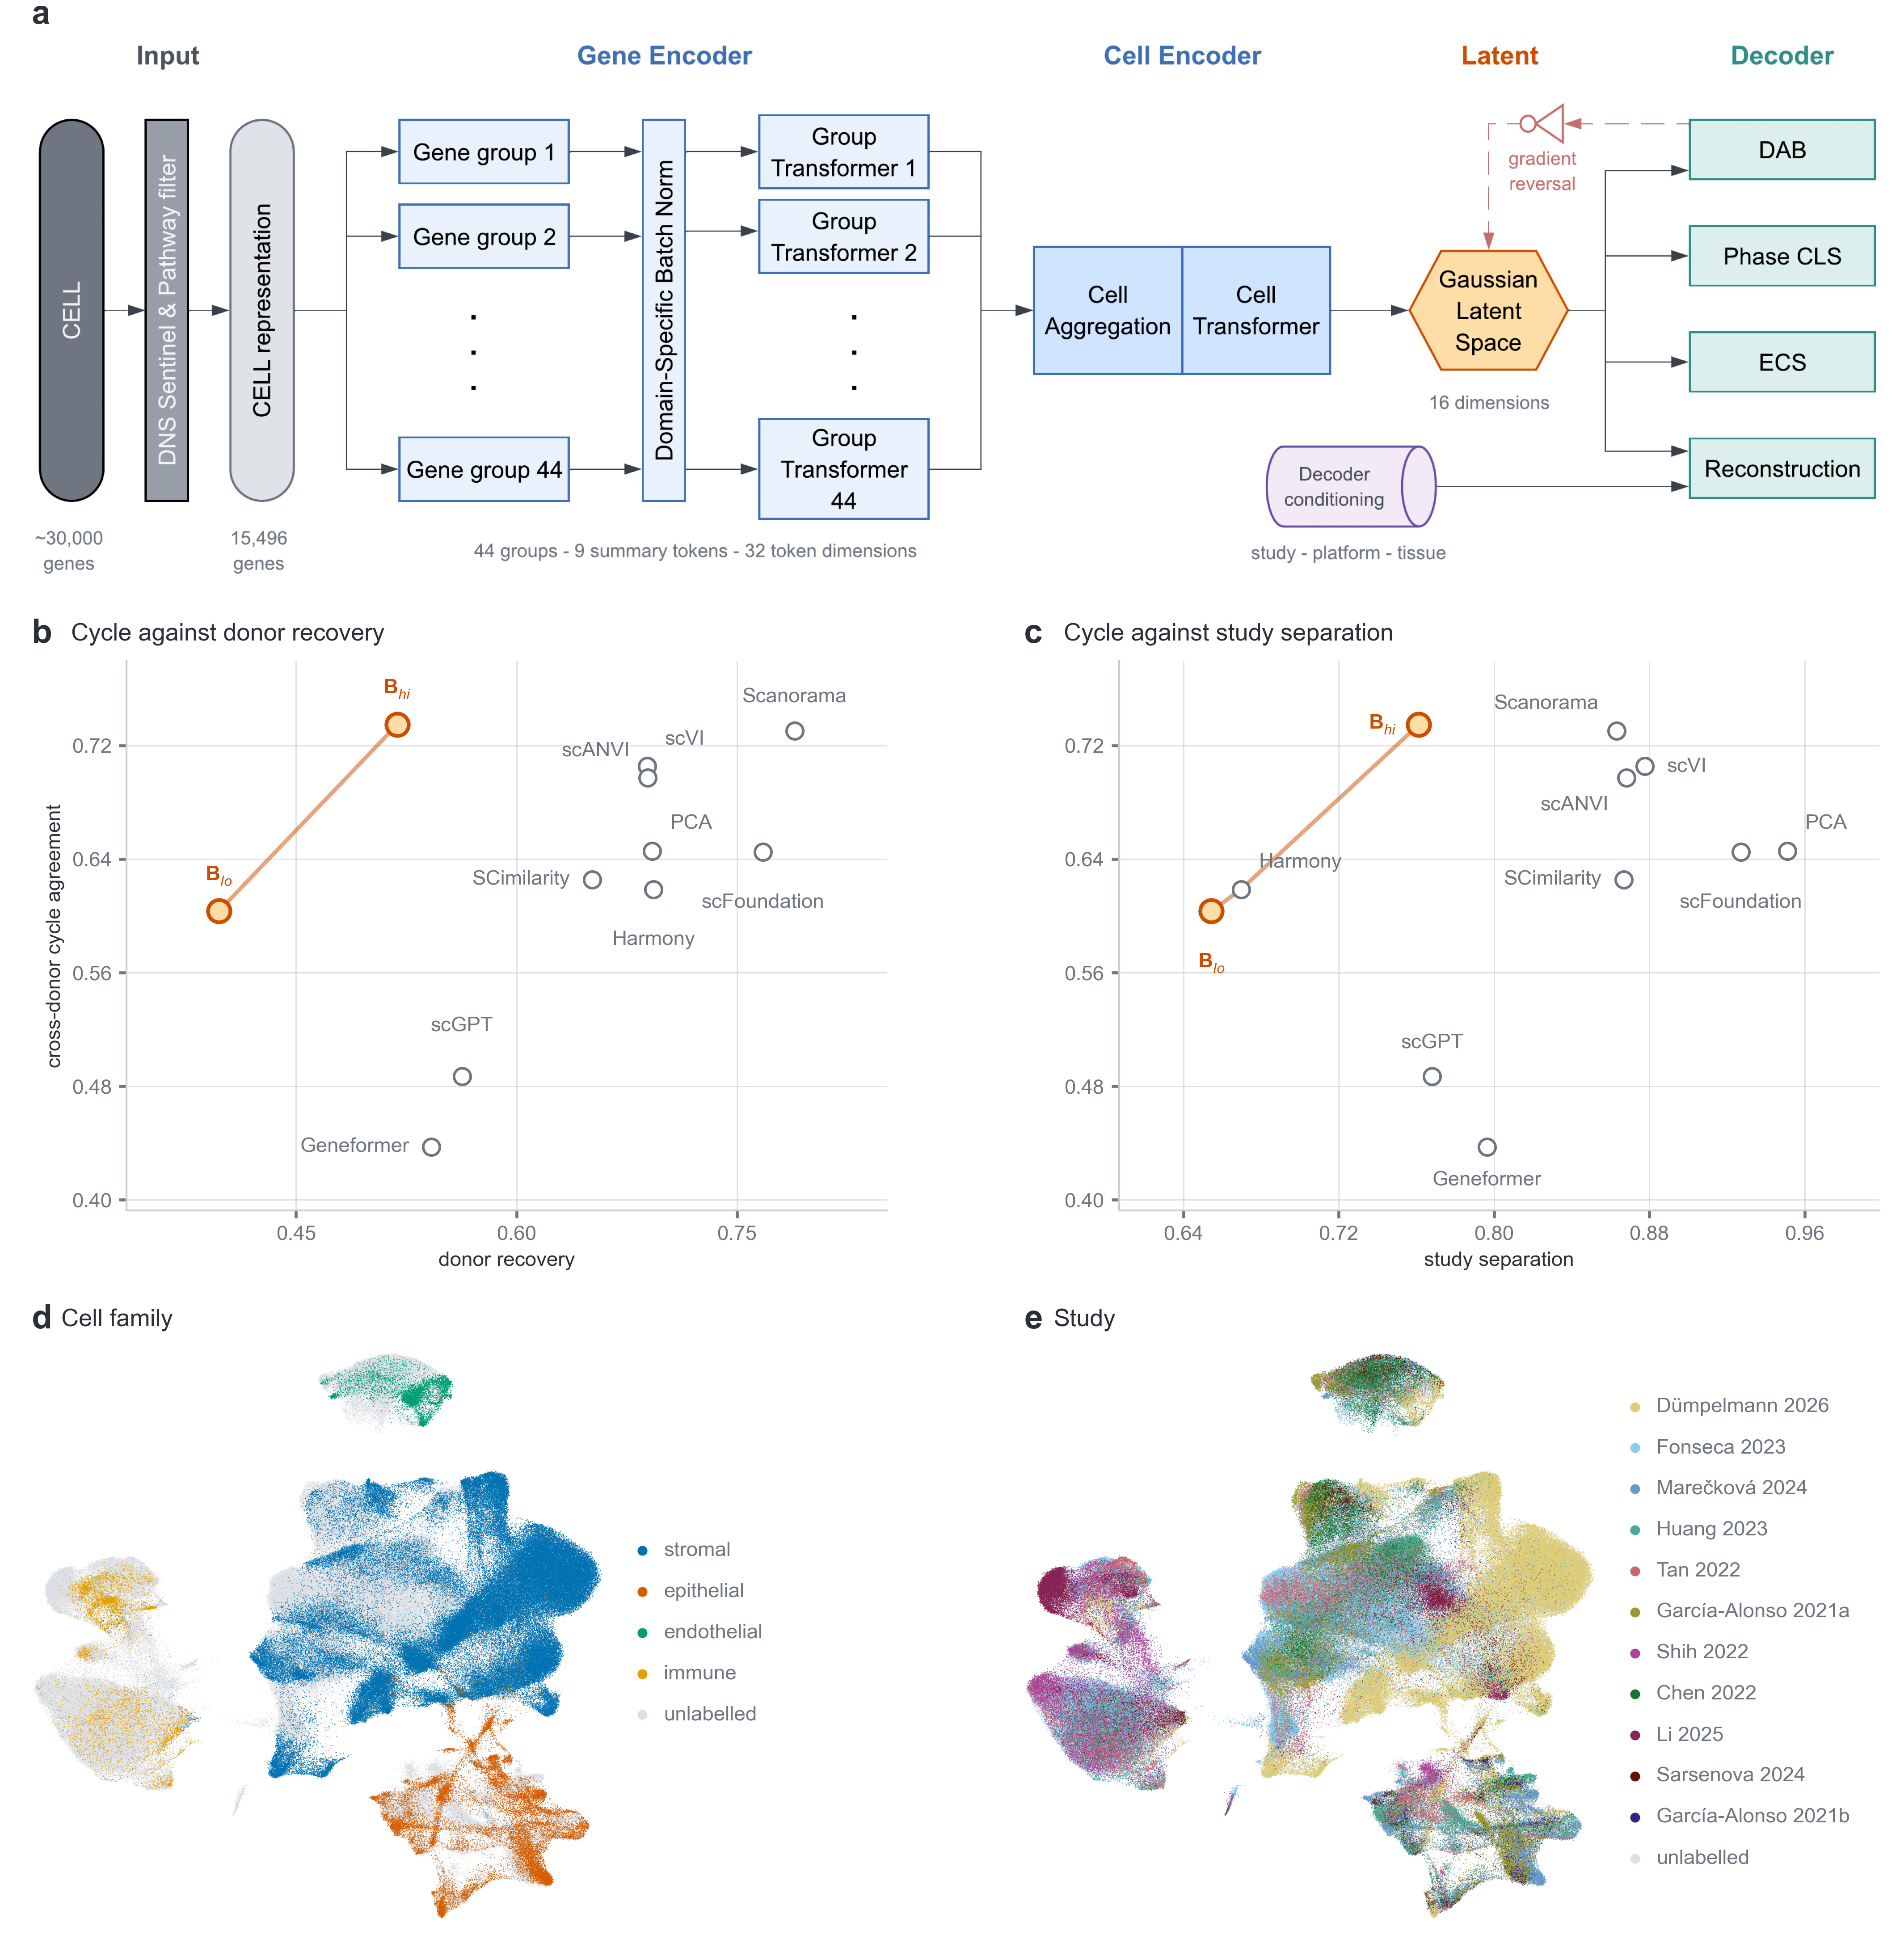
\includegraphics[width=\linewidth]{figures/pinned/figure1.png}
\caption{\textbf{\elaj\ pools eleven endometrial single-cell studies into
one sixteen-dimensional latent that keeps more cycle biology and less donor
identity than nine alternatives.} \textbf{a}, Overview. Data: every
eligible public study, drawn by its donor count (254 donors, 1{,}577{,}728
cells), with the corpus split by disease status. Model: the inductive biases
that replace pretraining scale. Outcomes: what the trained latent holds and
how it compares. \textbf{b}, Architecture. A cell enters as the genes shared
across the corpus, reduced to the 15{,}496 that map to one of 44 pathway
groups; a gene a study never assayed is carried by a did-not-sample (DNS)
sentinel, not a zero. Each group is normalised per study (domain-specific
batch normalisation, DSBN) and summarised by its own transformer into nine
tokens of 32 dimensions; a cell transformer compresses the 396 tokens to
sixteen Gaussian dimensions. Four heads read the latent: domain-adversarial
study removal (DAB), whose gradient is reversed on its way to the encoder;
reconstruction, conditioned on study, platform and site, which never reach
the encoder; elastic cell similarity (ECS); and a menstrual-phase classifier
(Phase CLS). Disease status is given to no part of the model.
\textbf{c}, Cross-donor agreement on menstrual phase against donor
recovery, both on the same held-out donors, for the two reported \elaj\
configurations (B$_{hi}$, B$_{lo}$, joined) and nine alternatives: five
integration and dimension-reduction methods and four pretrained foundation
models. Up and to the left is better. \textbf{d}, The B$_{hi}$ latent, 400{,}000
of all cells drawn at random, by cell family; cells without a family label
are grey. Uniform manifold approximation and projection (UMAP).}
\label{fig:model}
\end{figure}

\subsection*{Figure 2 --- How the two knobs move the frontier}
\note{THE P-SERIES ALONE, AND THE POINTS ARE JOINED. Figure 1 answers whether
\elaj\ is better, with every method and one Pareto front over the lot. This
one answers how the knobs work, so no baseline, no foundation model and no
ablation appears. Eight panels: two cost axes, two joining schemes, and two
rows of biology.
\\ROWS ARE CALIBRATED, NOT SHARED. Phase spans 0.1424 across these arms and
cell family 0.0288. Autoscaling each row makes the bottom look as dramatic as
the top, so the rows are pinned to 0.50--0.80 and 0.95--1.00 and labelled
once each. The bottom row is the control: the knobs trade phase against the
confounds and leave cell identity where it was.
\\CARRIES B1.
\\RENDERED at 1200 dpi.}

\begin{figure}[htbp]\centering
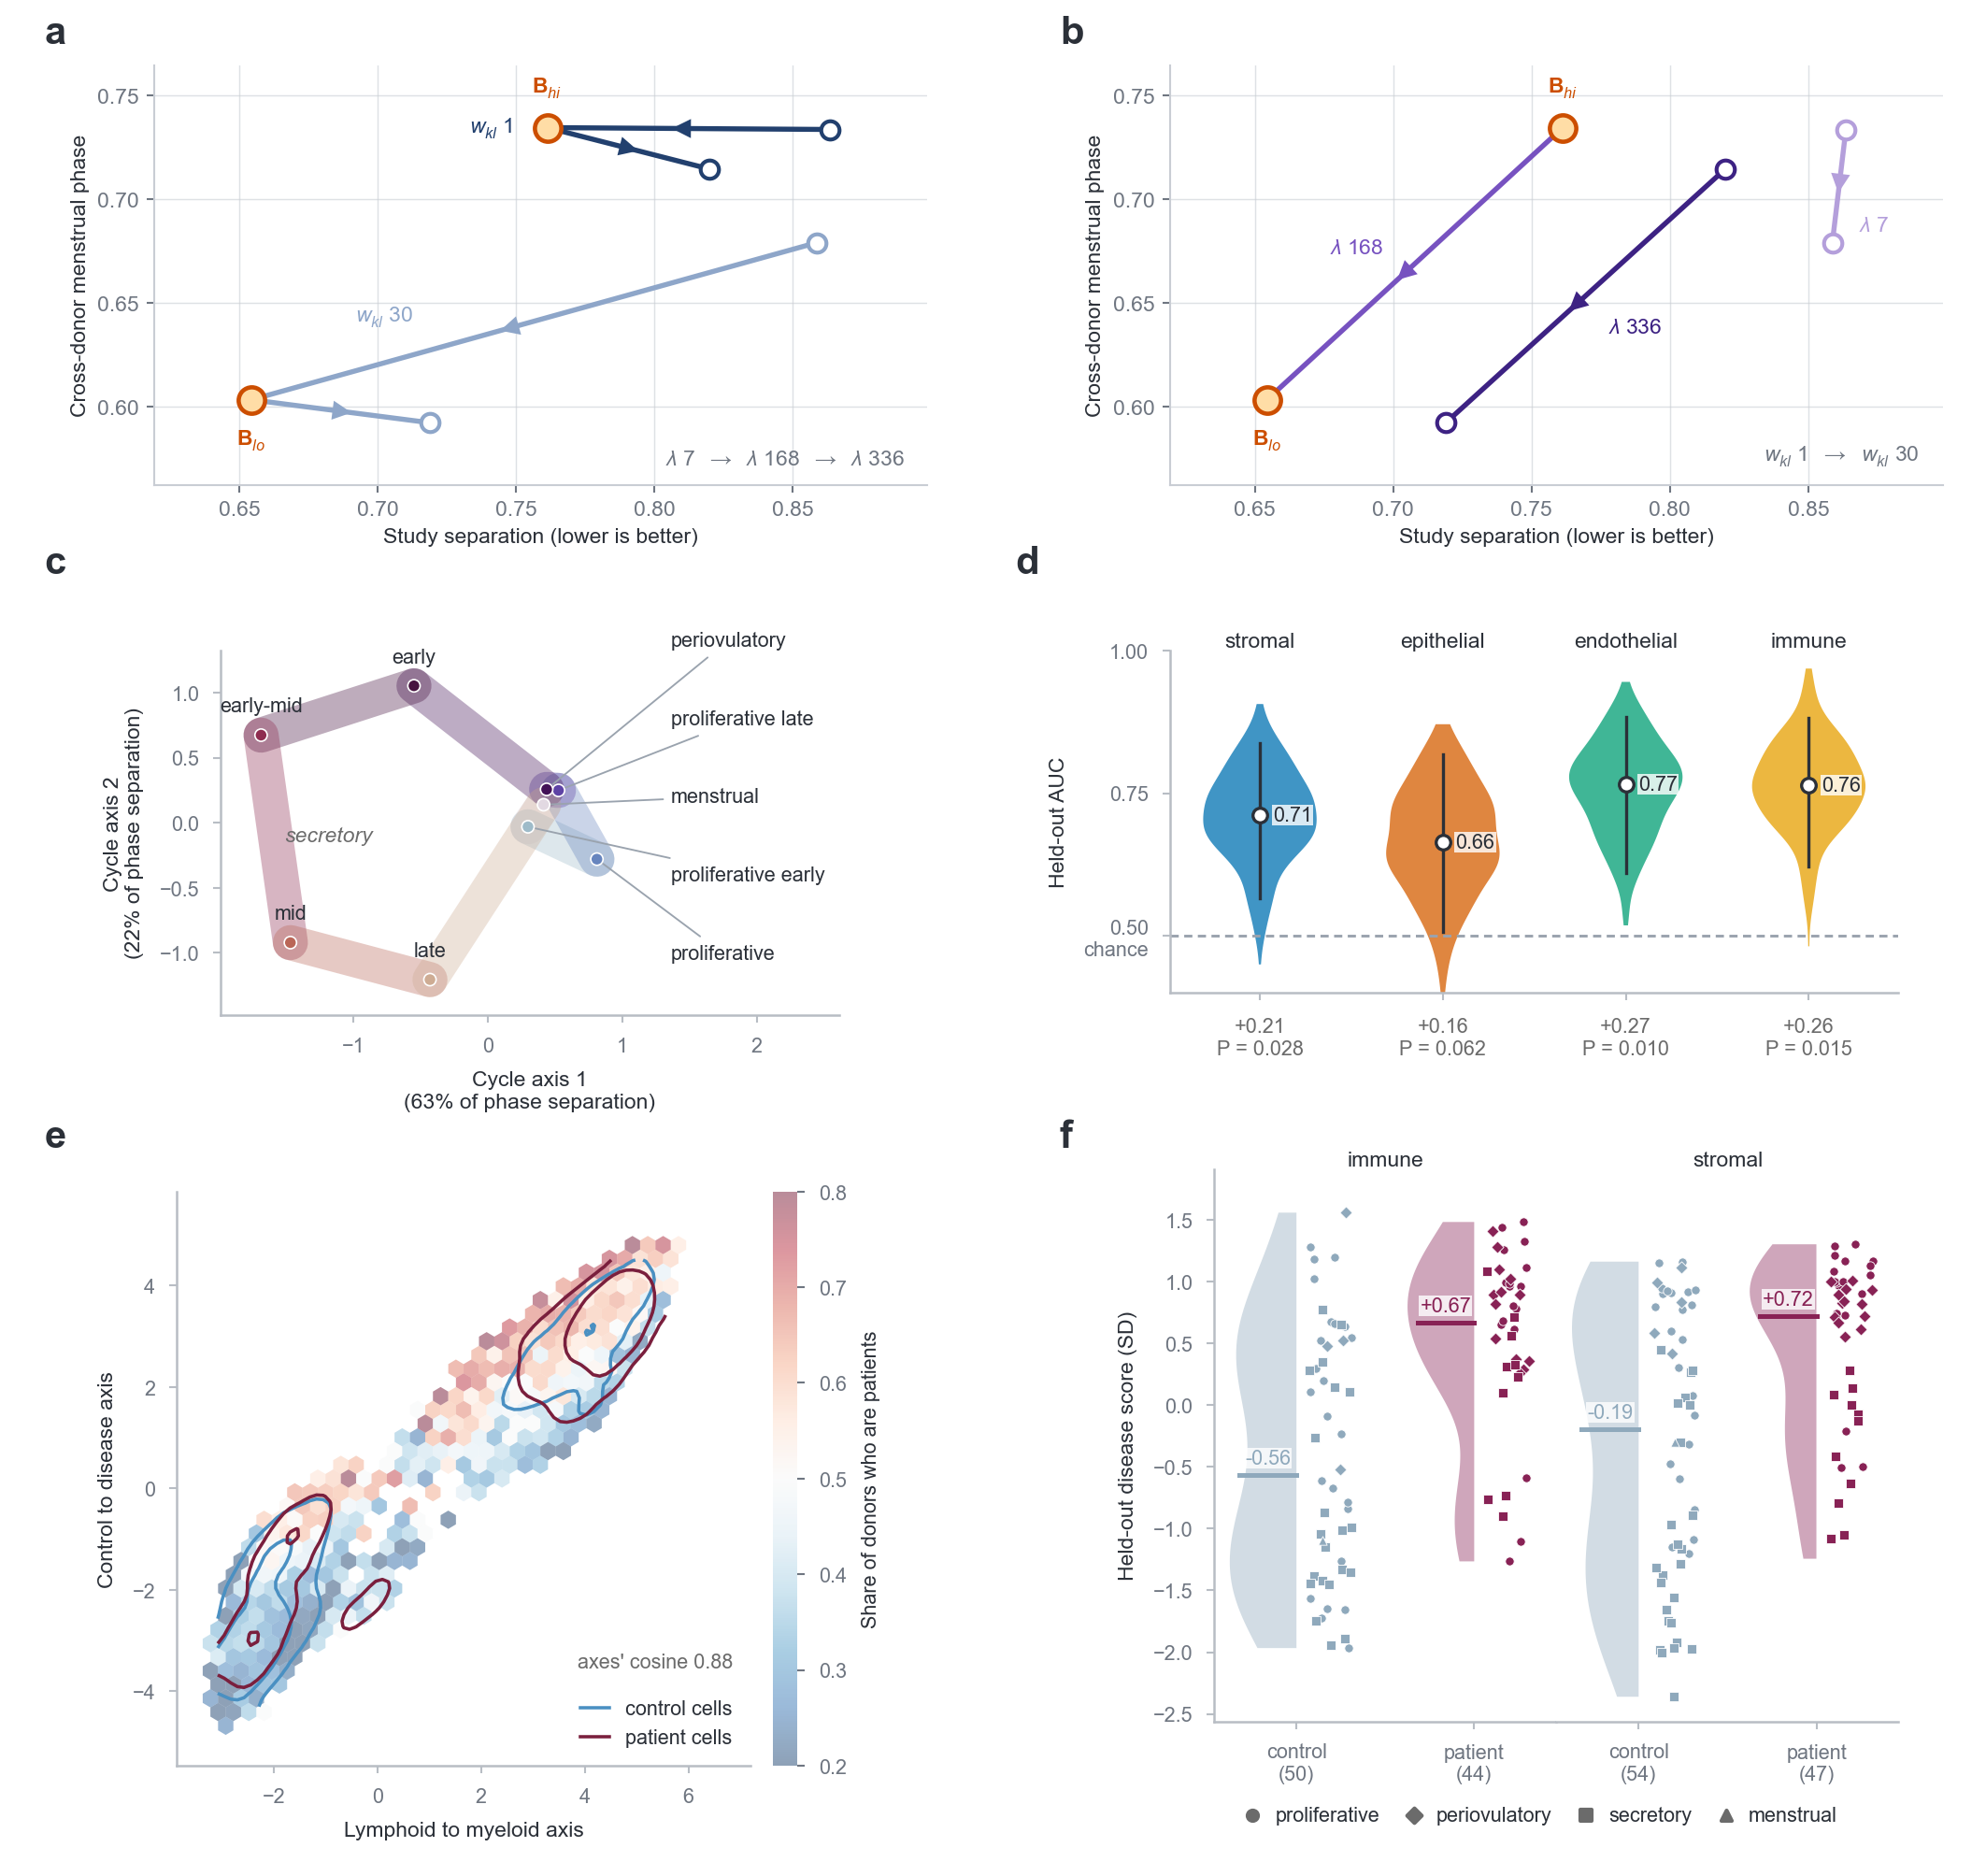
\includegraphics[width=\linewidth]{figures/pinned/figure2.png}
\caption{\textbf{Two coefficients set the trade-off, the latent closes the
cycle, and per-donor disease axes follow composition and the cycle.}
\textbf{a},~\textbf{b}, Six \elaj\ configurations, adversarial weight
$\lambda$ (7, 168, 336) crossed with information cost $w_{kl}$ (1, 30), by
study separation (lower is better) and cross-donor phase agreement. Lines
join equal $w_{kl}$ in \textbf{a}, arrows in order of rising $\lambda$, and
equal $\lambda$ in \textbf{b}. From $\lambda$ 7 to 168 study separation falls
from 0.86 to 0.76 at unchanged phase agreement (0.73); raising $w_{kl}$
moves every configuration along the trade-off. \textbf{c}, Centroids of the
nine harmonised phases on the first two linear discriminants of phase (63\%
and 22\% of the separation), joined in biological order by a band
coloured by stage: they advance round a closed loop (mean resultant length
0.80, permutation $P = 0.0018$). \textbf{d}, Disease status read from
held-out donors per cell family, as the area under the receiver operating
characteristic curve (AUC) over 400 70/30 donor splits: violin, the
splits; dot, median; line, 5th to 95th percentile; beneath, the median's
excess over chance (dashed) and permutation $P$. Stromal 101 donors,
epithelial 98, endothelial 85, immune 94. \textbf{e}, The 29{,}355 immune
cells two studies label lymphoid or myeloid, on the lymphoid-to-myeloid
axis and the immune disease axis (cosine 0.88). Hexagons, share of donors
who are patients, each counted once, blank below eight donors; blue and
dark red lines, the densest 20\% and 5\% of control and patient cells.
\textbf{f}, Each donor's held-out position on the immune and stromal
disease axes; shape, phase at biopsy; line and number, median; donors in
brackets. Secretory-phase donors sit at the control end whatever their
status. No step in \textbf{d}--\textbf{f} uses study, and disease status
was never given to the model.}
\label{fig:knobs}
\end{figure}

\subsection*{Figure 3 --- Both latents, by cell family and cycle phase}
\note{TEN PANELS, two arms by five columns. \textbf{a}--\textbf{e}
ELAJ$_{B\,hi}$, \textbf{f}--\textbf{j} ELAJ$_{B\,lo}$; columns are all
labelled cells, then stromal, epithelial, endothelial and immune. Phase in the
animation's five-group palette, cells of other families drawn in grey so each
panel keeps the whole embedding's shape.
\\WHERE A READER MEETS BOTH LATENTS SIDE BY SIDE and can judge for themselves
that $B\,hi$ holds phase territories $B\,lo$ smears. No annotation says so.
\\MENSTRUATION IS EXCLUDED HERE and shown in Figure 4, because this figure
reads the cycle axis and \texttt{groupings.py} rules that menstruation is a
distinct state rather than a point on it.
\\RENDERED, all 1{,}577{,}728 cells sampled to 400{,}000 for the scatter.}

\begin{figure}[htbp]\centering
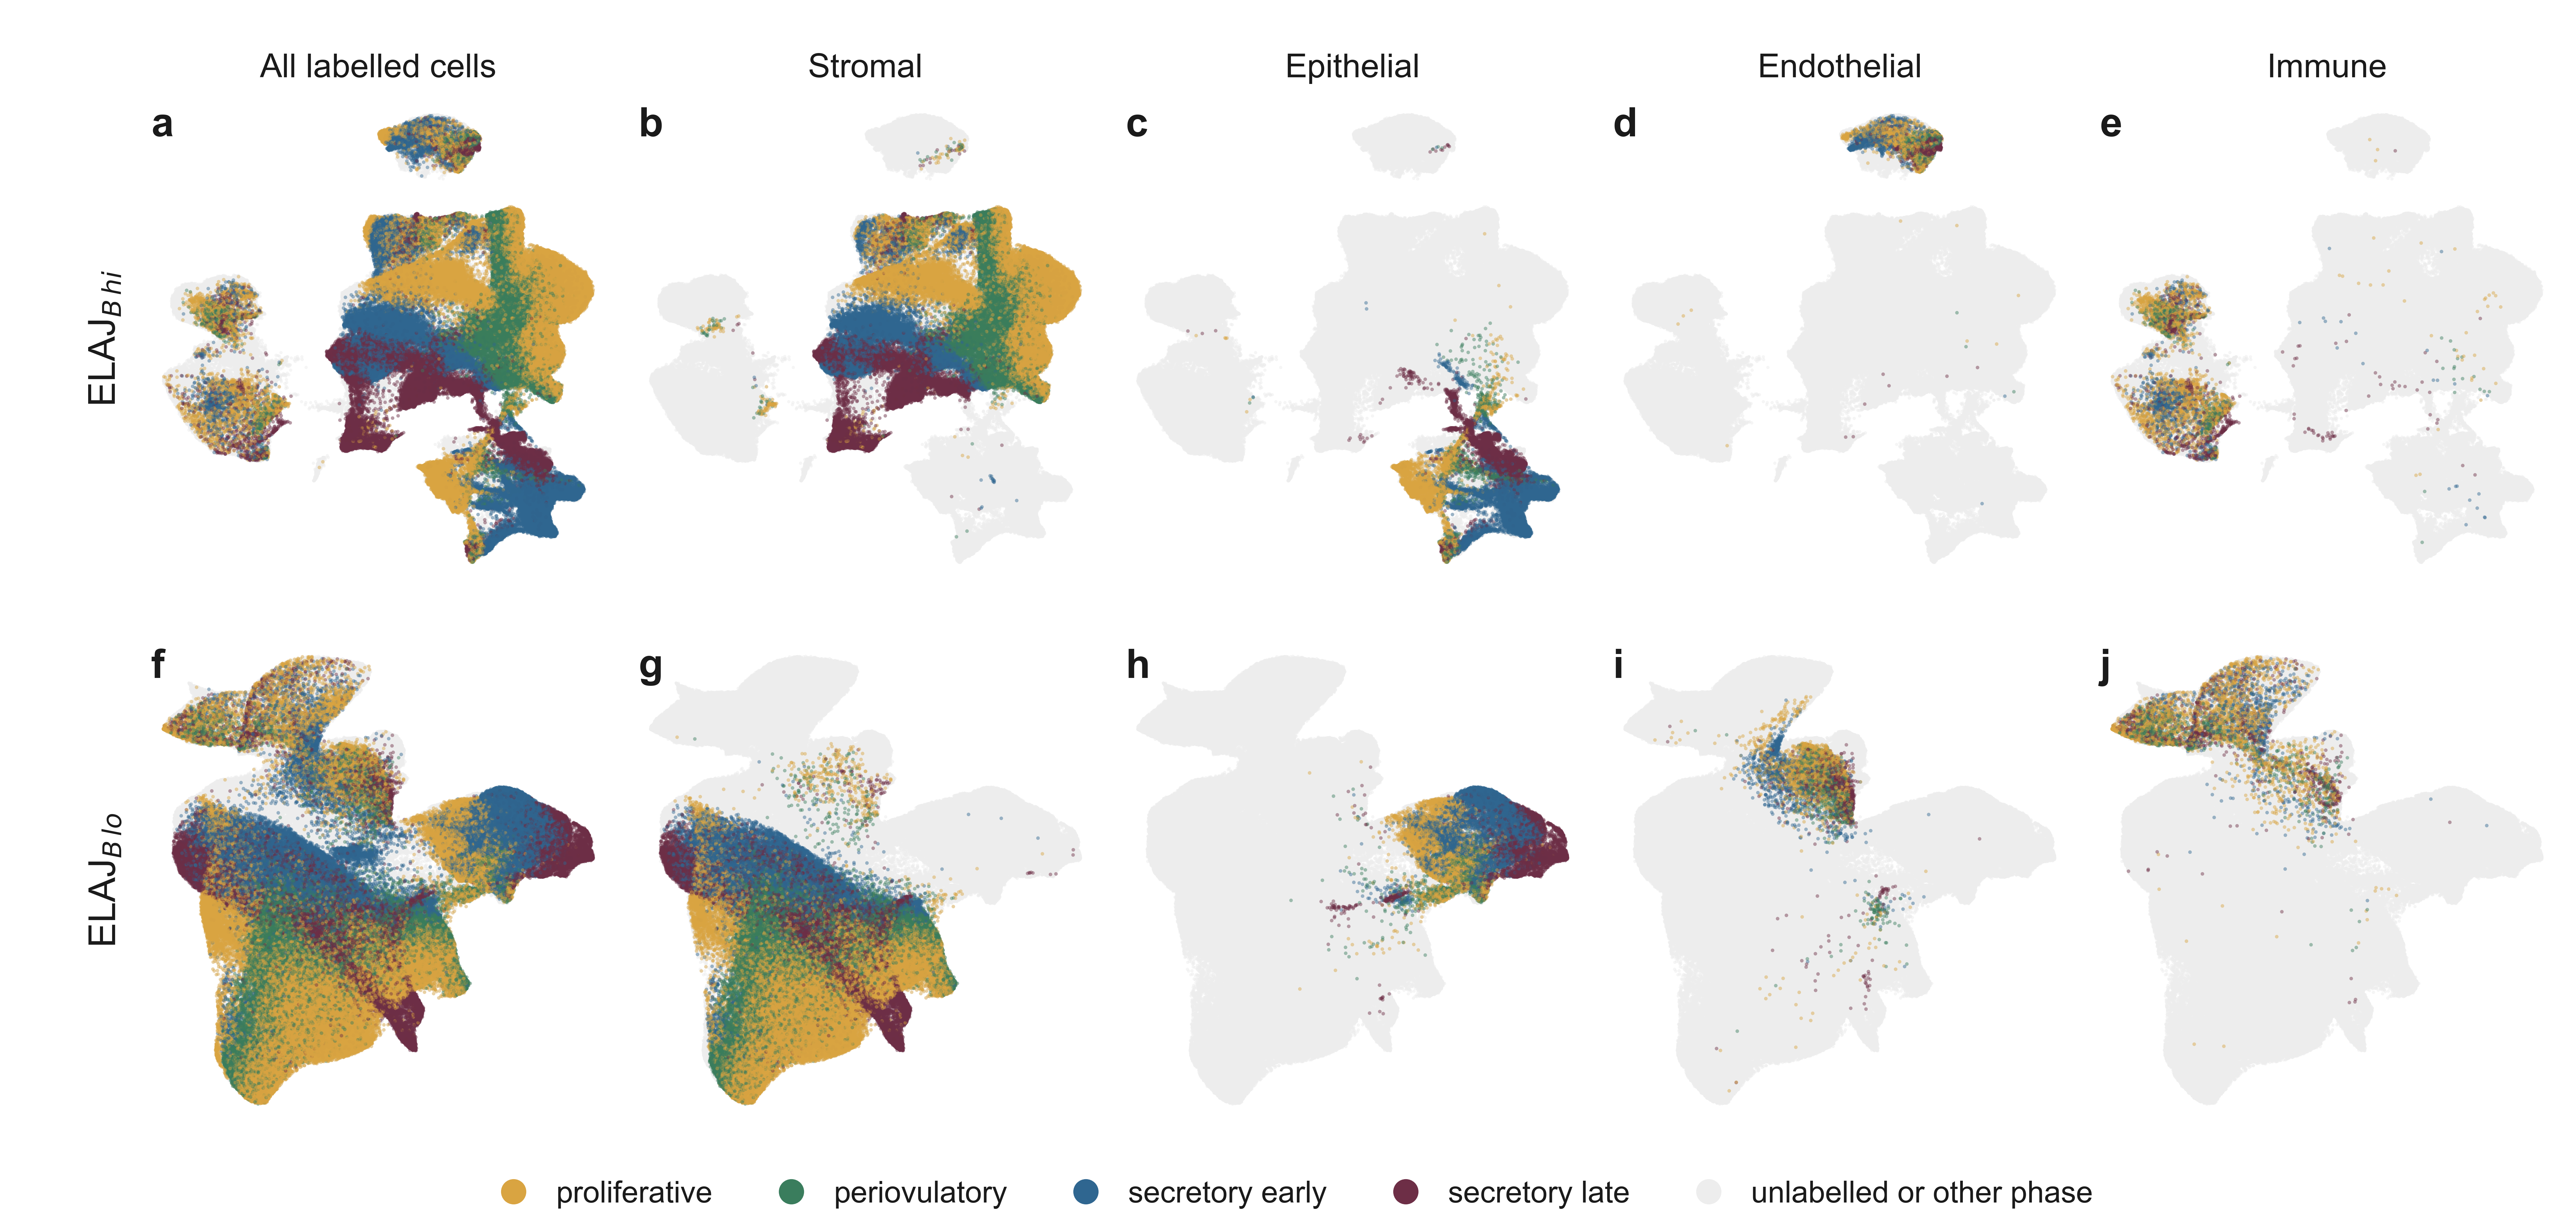
\includegraphics[width=\linewidth]{figures/pinned/figure3.png}
\caption{\textbf{\elaj\ models by cell family and cycle phase.} Every
panel is a UMAP of the same sixteen-dimensional latent, showing 400{,}000
cells drawn at random to limit overplotting. The 
top row (\textbf{a}--\textbf{e}) represents ELAJ$_{B\,hi}$ while the bottom 
row (\textbf{f}--\textbf{j}) represents ELAJ$_{B\,lo}$. The two arms differ 
only in their adversarial and KL weights. Columns represent cell family: 
all labelled cells (\textbf{a},~\textbf{f}), stromal (\textbf{b},
~\textbf{g}), epithelial (\textbf{c},~\textbf{h}), endothelial (\textbf{d},
~\textbf{i}) and immune (\textbf{e},~\textbf{j}). Colour is harmonised 
menstrual phase in four groups; cells with no phase label, and cells of 
another family in that column, are drawn in grey. Menstruation is excluded 
here as it carries fewer than 4{,}199 cells and is a distinct physiological 
state rather than a point on the proliferative-to-secretory axis.
\\The contrast between the rows is the frontier of Figure~2 made visible.
ELAJ$_{B\,hi}$ holds the phases as contiguous territories; ELAJ$_{B\,lo}$,
which removes study signal substantially better, smears them. Nothing
separates the two arms but the weight on each objective.
\\The contrast between the columns is the cell-type split of the cycle.
Cycle structure is sharp in stromal cells, present in
epithelial, and close to absent in endothelial and immune, which is the order
in which those compartments remodel across the cycle. The phase head is a
single linear map over the whole latent and was never given cell family, so a
split of the cycle by cell type is not something the supervision could have
produced.}
\label{fig:latents}
\end{figure}

\subsection*{Figure 4 --- What endometriosis looks like, in nine UMAPs}
\note{NINE PANELS over the whole corpus, one embedding, nine colourings:
\textbf{a} study, \textbf{b} tissue, \textbf{c} menstrual phase,
\textbf{d} cycle day, \textbf{e} serum progesterone, \textbf{f} the X16
cycle axis, \textbf{g} disease status, \textbf{h} merged severity,
\textbf{i} surgical stage.
\\RESTRUCTURED 17 NOVEMBER on AW's ruling: cell family removed (Figure 1d
already shows it), the old b--f moved up one, and the cycle axis added at
\textbf{f}, so the second row is the cycle read three ways, two measured by
the clinic and one held by the latent. The axis is the X16 discriminant,
imported from \texttt{supp\_figures.\_cycle\_setup}, and the render
reproduces $\rho$ = 0.7565 against cycle day.
\\Grade was dropped on AW's ruling of 6 November: it is a coarsening of
the same rASRM scale. The merged severity column is built by importing the
project's own harmoniser rather than retyping the mapping. Each title
carries the share of cells the label covers.
\\CARRIES C4 and C5, and the staging result visually: \textbf{h} and
\textbf{i} show no structure that any of the other panels show.
\\ONE SHARED SHUFFLED Z-ORDER across every panel.
\\RENDERED, 400{,}000 of 1{,}577{,}728 cells, no split restriction, which is
correct because none of these labels is a model input.}

\begin{figure}[htbp]\centering
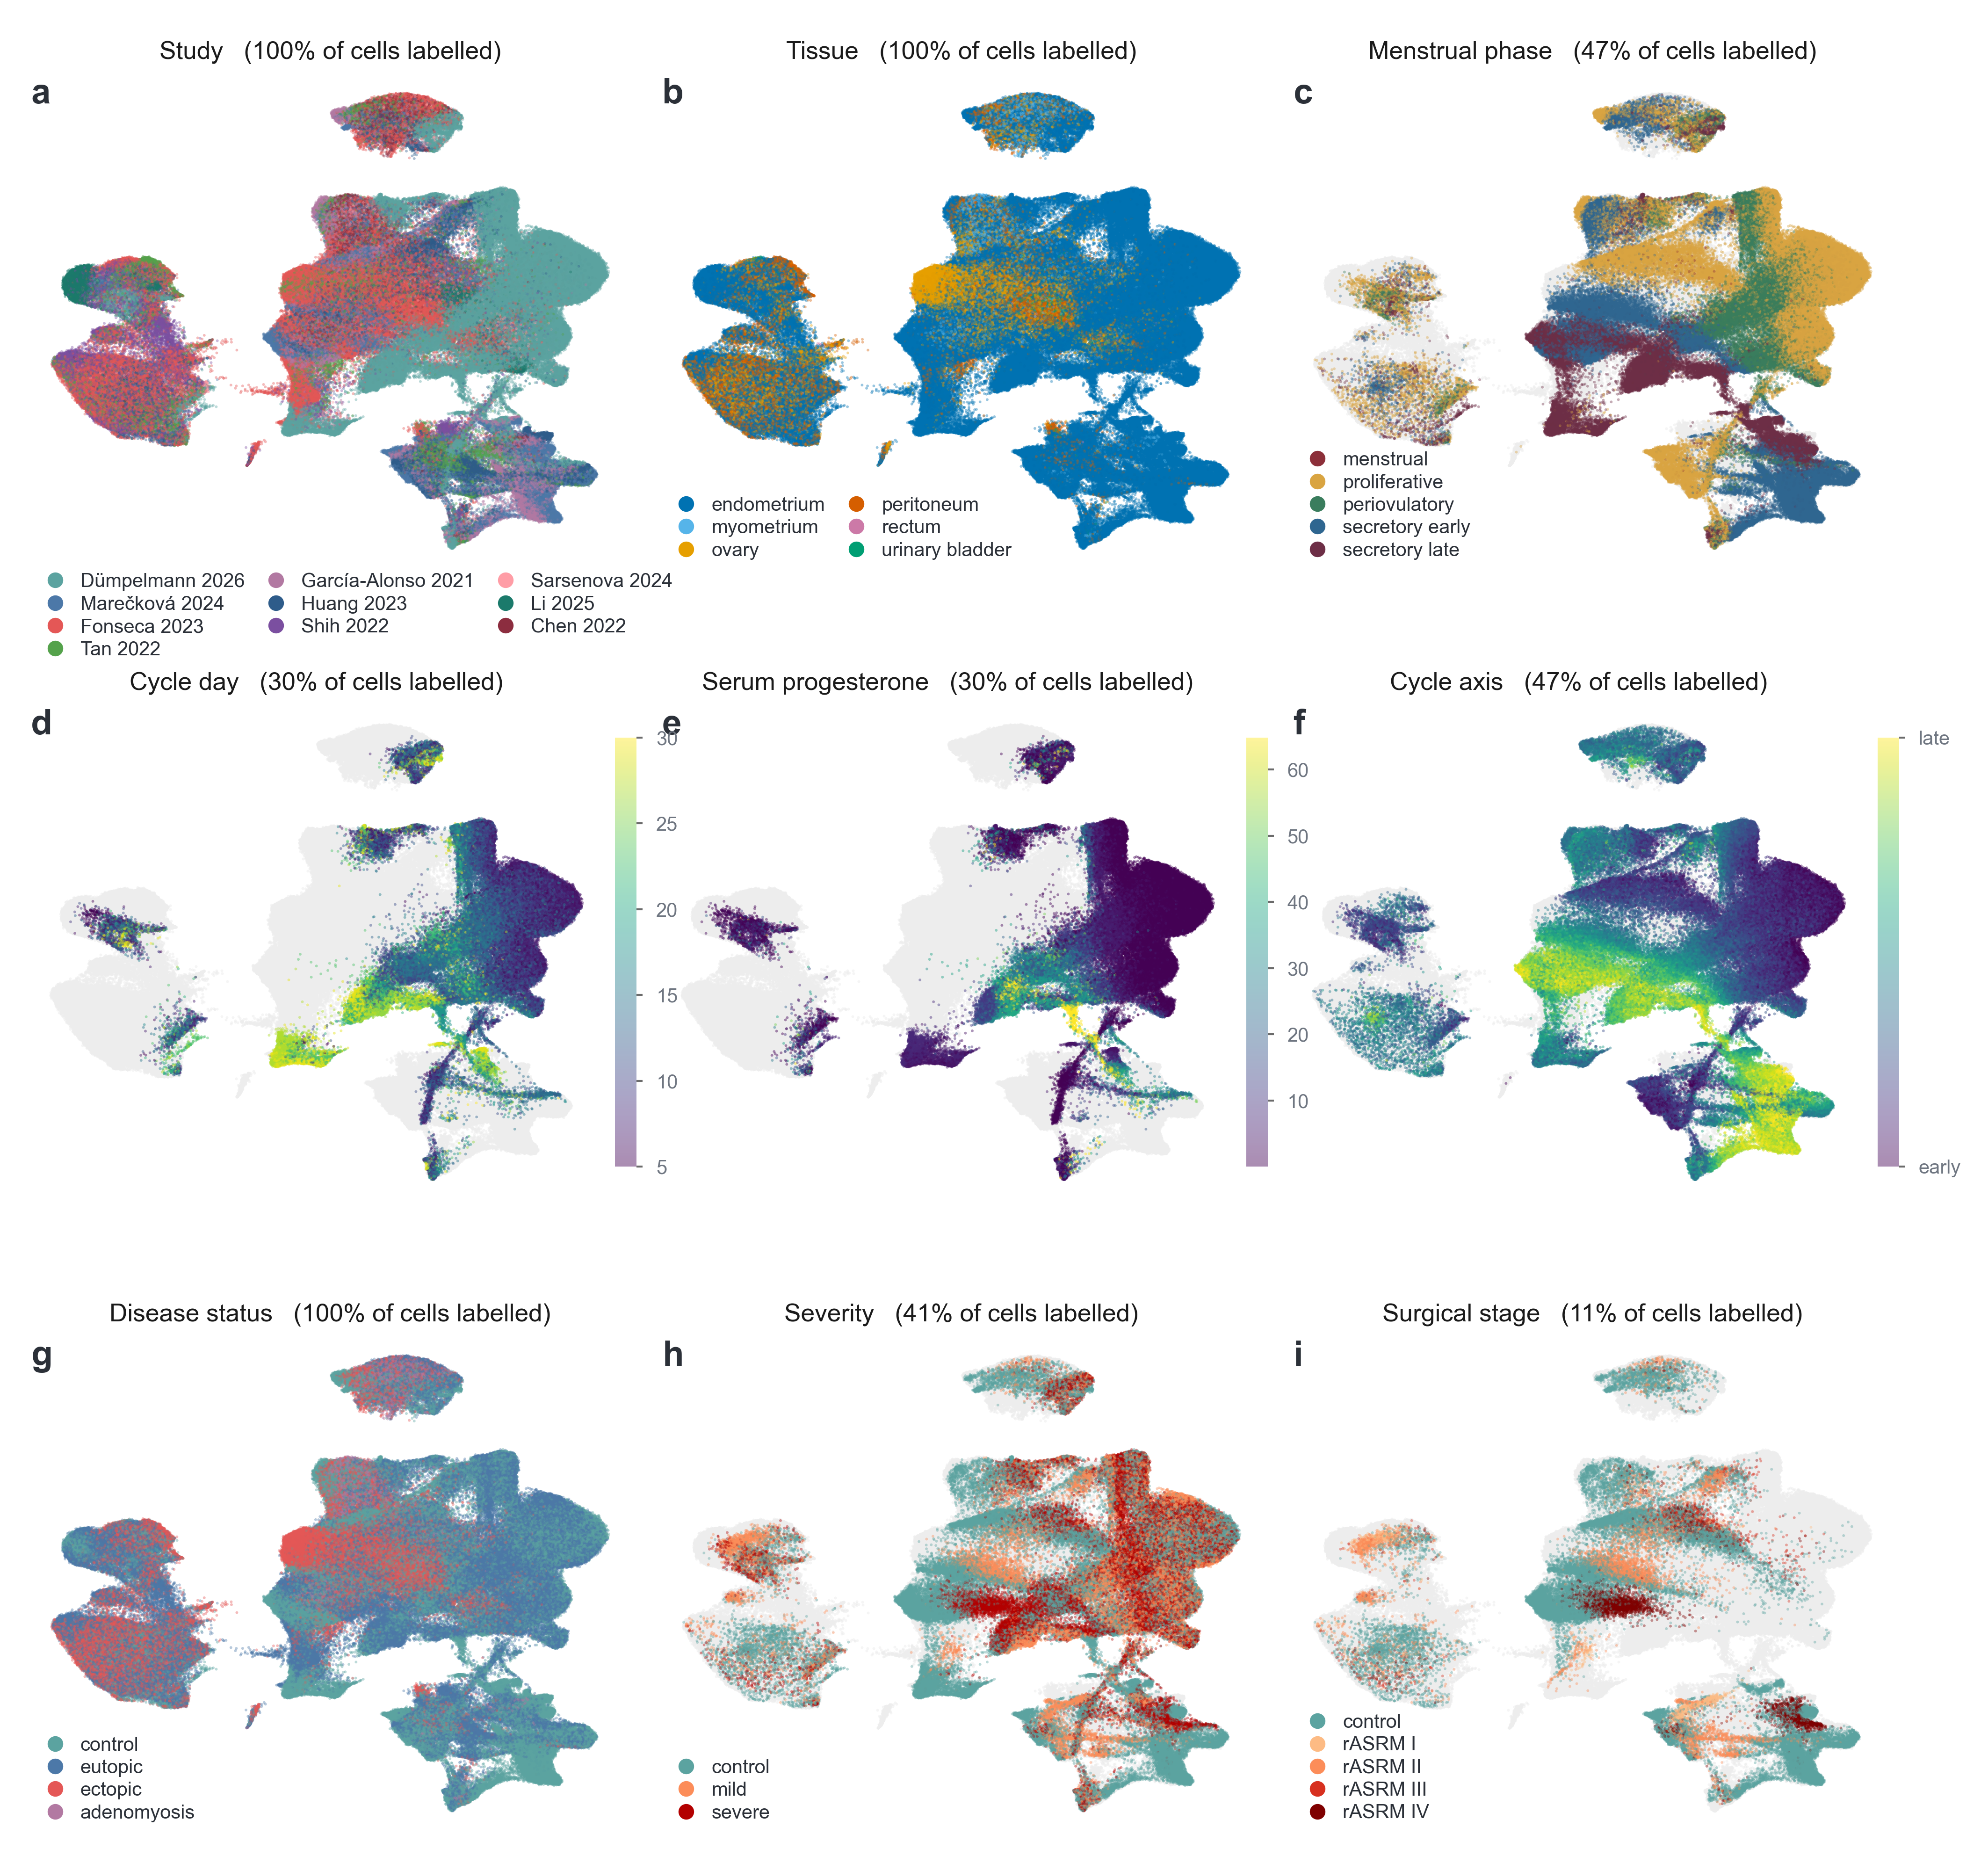
\includegraphics[width=\linewidth]{figures/pinned/figure4.png}
\caption{\textbf{Endometriosis viewed through \elaj.} All panels show the 
UMAP of ELAJ$_{B\,hi}$'s sixteen-dimensional latent, 400{,}000 cells drawn at
random, recoloured by one variable each: study (\textbf{a}), anatomical
site (\textbf{b}), harmonised menstrual phase (\textbf{c}), cycle day
(\textbf{d}), serum progesterone (\textbf{e}), position on the cycle axis
(\textbf{f}), disease status (\textbf{g}), merged severity (\textbf{h}) and
surgical stage (\textbf{i}). Each title gives the share of cells carrying
that label, and cells without it are drawn in grey. The cycle axis in
\textbf{f} is a single linear direction in the latent, fitted to the phase
labels of two cohorts and never to \texttt{duempelmann\_2026}, the only
cohort recording cycle day and progesterone; it is drawn on phase-labelled
cells and runs from early to late in the cycle. Severity in \textbf{h} merges the two
cohorts' vocabularies onto one three-level scale; rASRM I--II are mild, 
rASRM III--IV are severe. Of the nine variables only menstrual phase was 
supplied to the model, through one supervised head.
\\Cycle day (\textbf{d}), serum progesterone (\textbf{e}) and the cycle
axis (\textbf{f}) trace one gradient, the cycle as a continuum, held along a
direction that orders a cohort it was never fitted on. Merged severity
(\textbf{h}) and surgical stage (\textbf{i}) organise nothing, as in all ten
representations tested. Study (\textbf{a}) and site (\textbf{b}), both
decoder covariates, retain visible structure.}
\label{fig:endo}
\end{figure}

\subsection*{Table 1 --- Every representation on every axis}
\note{REPLACES FIGURE 5, on AW's ruling of 6 November. The five-panel
ablations figure becomes one long table over the p-series, the a-series,
the baselines and the foundation models. NMI counts a table as a display
item, so the paper stays at five of six.
\\GENERATED, never typed: \texttt{figures/scripts/table1.py} reads the same
files the two auditors read, so a cell here and the same number in the
prose cannot come from different runs. Regenerate after any re-score.
\\ORDERING IS THE ARGUMENT. Four blocks, each sorted by cross-donor
menstrual phase descending, so a reader meets every group at its best. The
ablations are the exception: the base leads, because the rest are
single-key changes against it.
\\CARRIES D1--D6 and the whole field comparison. B2 and B3 are not here;
they were cut from Results \texttt{[6]} and from the Discussion.}

% GENERATED by figures/scripts/table1.py. Do not edit by hand.
\begin{table*}[p]\centering\footnotesize
\setlength{\tabcolsep}{3pt}
\caption{\textbf{Every representation on every axis.} Cross-donor agreement, reported as excess over chance, for menstrual phase, cell family and merged severity; $k$-nearest-neighbour agreement for the forty-five-way cell type and for donor identity; pooled control-against-eutopic agreement for disease; and $k$NN study purity for study separation, rescaled so that 0 is perfectly mixed and 1 fully separated. $\uparrow$ marks an axis where more is better and $\downarrow$ one where less is. Held-out split throughout. \texttt{val\_nb} is held-out negative-binomial reconstruction loss per cell at the selected checkpoint, which only the \elaj\ arms have. Rows are ordered within each block by cross-donor menstrual phase, except the ablations, where the base arm leads because the rest are single-key changes against it. $\lambda$ is the adversarial weight and $w_{kl}$ the information cost. Every value is on the same held-out donors. \\The table is read down the biology columns and across to the cost ones. Four blocks: the six-arm grid that traces the frontier, the five single-key ablations against ELAJ$_{B\,hi}$, five integration and dimension-reduction methods, and four pretrained foundation models. Two readings it is meant to support. Cell family separates nine of the ten methods by 0.0076, so cell identity is something every representation recovers and none can be ranked on, while menstrual phase spans 0.4372 to 0.7397 across the same rows. And the arm with the best reconstruction in the table, the shuffled gene grouping at 0.3911, holds the least disease signal in it.}
\label{tab:field}
\begin{tabular}{l r l rrrrr rr r}
\toprule
 & & & \multicolumn{5}{c}{\textbf{biology} $\uparrow$} & \multicolumn{2}{c}{\textbf{cost} $\downarrow$} & \\
\cmidrule(lr){4-8}\cmidrule(lr){9-10}
model & dims & super- & phase & cell & cell & disease & sever- & donor & study & \texttt{val\_nb} \\
 & & vised on & & family & type & & ity & & & $\downarrow$ \\
\midrule
\multicolumn{11}{l}{\textit{\elaj, the two knobs}} \\
\textbf{$\lambda$ 168, $w_{kl}$ 1\,(B\textsubscript{hi})} & 16 & phase & \textbf{0.7346} & \textbf{0.9820} & \textbf{0.4964} & \textbf{0.3364} & \textbf{0.1157} & \textbf{0.5188} & \textbf{0.7613} & 0.4024 \\
$\lambda$ 7, $w_{kl}$ 1 & 16 & phase & 0.7337 & 0.9829 & 0.5043 & 0.3449 & 0.1195 & 0.5837 & 0.8636 & 0.4016 \\
$\lambda$ 336, $w_{kl}$ 1 & 16 & phase & 0.7146 & 0.9779 & 0.4890 & 0.3558 & 0.0950 & 0.5277 & 0.8200 & 0.3991 \\
$\lambda$ 7, $w_{kl}$ 30 & 16 & phase & 0.6791 & 0.9841 & 0.4834 & 0.3483 & 0.1304 & 0.5389 & 0.8587 & 0.4025 \\
\textbf{$\lambda$ 168, $w_{kl}$ 30\,(B\textsubscript{lo})} & 16 & phase & \textbf{0.6033} & \textbf{0.9565} & \textbf{0.4442} & \textbf{0.3045} & \textbf{0.1155} & \textbf{0.3975} & \textbf{0.6544} & 0.4046 \\
$\lambda$ 336, $w_{kl}$ 30 & 16 & phase & 0.5922 & 0.9553 & 0.4477 & 0.3304 & 0.1245 & 0.4154 & 0.7190 & 0.4023 \\
\midrule
\multicolumn{11}{l}{\textit{\elaj, one key changed against B\textsubscript{hi}}} \\
B\textsubscript{hi}, unchanged & 16 & phase & 0.7346 & 0.9820 & 0.4964 & 0.3364 & 0.1157 & 0.5188 & 0.7613 & 0.4024 \\
no ECS & 16 & phase & 0.7397 & 0.9837 & 0.4994 & 0.3638 & 0.1232 & 0.5520 & 0.8340 & 0.4004 \\
no DNS sentinel & 16 & phase & 0.7308 & 0.9816 & 0.4944 & 0.3615 & 0.1047 & 0.5207 & 0.7818 & 0.4005 \\
random gene grouping & 16 & phase & 0.6780 & 0.9606 & 0.4889 & 0.2698 & 0.0572 & 0.5323 & 0.7701 & 0.3911 \\
no order statistics & 16 & phase & 0.6384 & 0.9798 & 0.4826 & 0.3225 & 0.1158 & 0.4943 & 0.7600 & 0.3979 \\
no phase head & 16 & -- & 0.4812 & 0.9794 & 0.4536 & 0.3170 & 0.1429 & 0.3754 & 0.6523 & 0.4083 \\
\midrule
\multicolumn{11}{l}{\textit{integration and dimension reduction}} \\
Scanorama$^{\dagger}$ & 100 & -- & 0.7303 & 0.9866 & 0.5516 & 0.4290 & 0.1505 & 0.7892 & 0.8632 & -- \\
scVI & 16 & -- & 0.7053 & 0.9828 & 0.5308 & 0.3689 & 0.0789 & 0.6888 & 0.8776 & -- \\
scANVI & 16 & cell family & 0.6971 & 0.9832 & 0.5333 & 0.3481 & 0.0759 & 0.6893 & 0.8683 & -- \\
PCA & 16 & -- & 0.6457 & 0.9866 & 0.5065 & 0.3640 & 0.1408 & 0.6923 & 0.9510 & -- \\
Harmony$^{\dagger}$ & 50 & -- & 0.6186 & 0.9823 & 0.5457 & 0.3846 & 0.1250 & 0.6932 & 0.6697 & -- \\
\midrule
\multicolumn{11}{l}{\textit{pretrained foundation models}} \\
scFoundation & 3072 & -- & 0.6449 & 0.9832 & 0.5366 & 0.4024 & 0.1695 & 0.7675 & 0.9272 & -- \\
SCimilarity & 128 & cell family & 0.6255 & 0.9896 & 0.5282 & 0.3646 & 0.1416 & 0.6516 & 0.8669 & -- \\
scGPT & 512 & -- & 0.4869 & 0.9840 & 0.4729 & 0.3473 & 0.1323 & 0.5630 & 0.7682 & -- \\
Geneformer & 256 & -- & 0.4372 & 0.9023 & 0.4136 & 0.3713 & 0.1860 & 0.5421 & 0.7964 & -- \\
\bottomrule
\end{tabular}
\\[2pt]\footnotesize $^{\dagger}$ fitted transductively on the cells it is scored on; every other method was fitted on the training donors and applied to held-out ones.
\end{table*}


\section*{Extended Data}
\note{TEN MAXIMUM (NMI, Preparing your material). Captions here carry the
detail main-text captions cannot afford. Allocation, in priority order:
\\1. The whole-corpus versus cross-donor inversion --- E1, the
$\rho$ +0.943 table and \texttt{random groups} going best-of-six to
worst-of-six. The strongest evidence for our own estimator.
\\2. The same-donor floor --- E2, per label, with the chance rate beside
it.
\\3. The remaining crop panels: phase, stage, grade, platform,
progesterone.
\\4. The donor-overlap audit --- 17{,}873 cells, 4.3\%, one study pair.
\\5. Baseline fitting: inductive versus transductive, per method, with
\texttt{supervised\_on}.
\\6. Per-arm comparison tables across the full factorial.
\\7. Sufficient-statistics tables at every coarsening.
\\8--10. Held.}

\subsection*{Extended Data Fig.~1 --- Record selection}
\note{MOVED OUT OF FIGURE 1 on AW's ruling of 10 November. It was panel b, a
tall column down the left, and it was why that figure carried three column
structures and no air. PRISMA is reporting apparatus rather than a finding.
\\Generated by \texttt{figures/scripts/extdata1\_prisma.py}.}

\begin{figure}[htbp]\centering
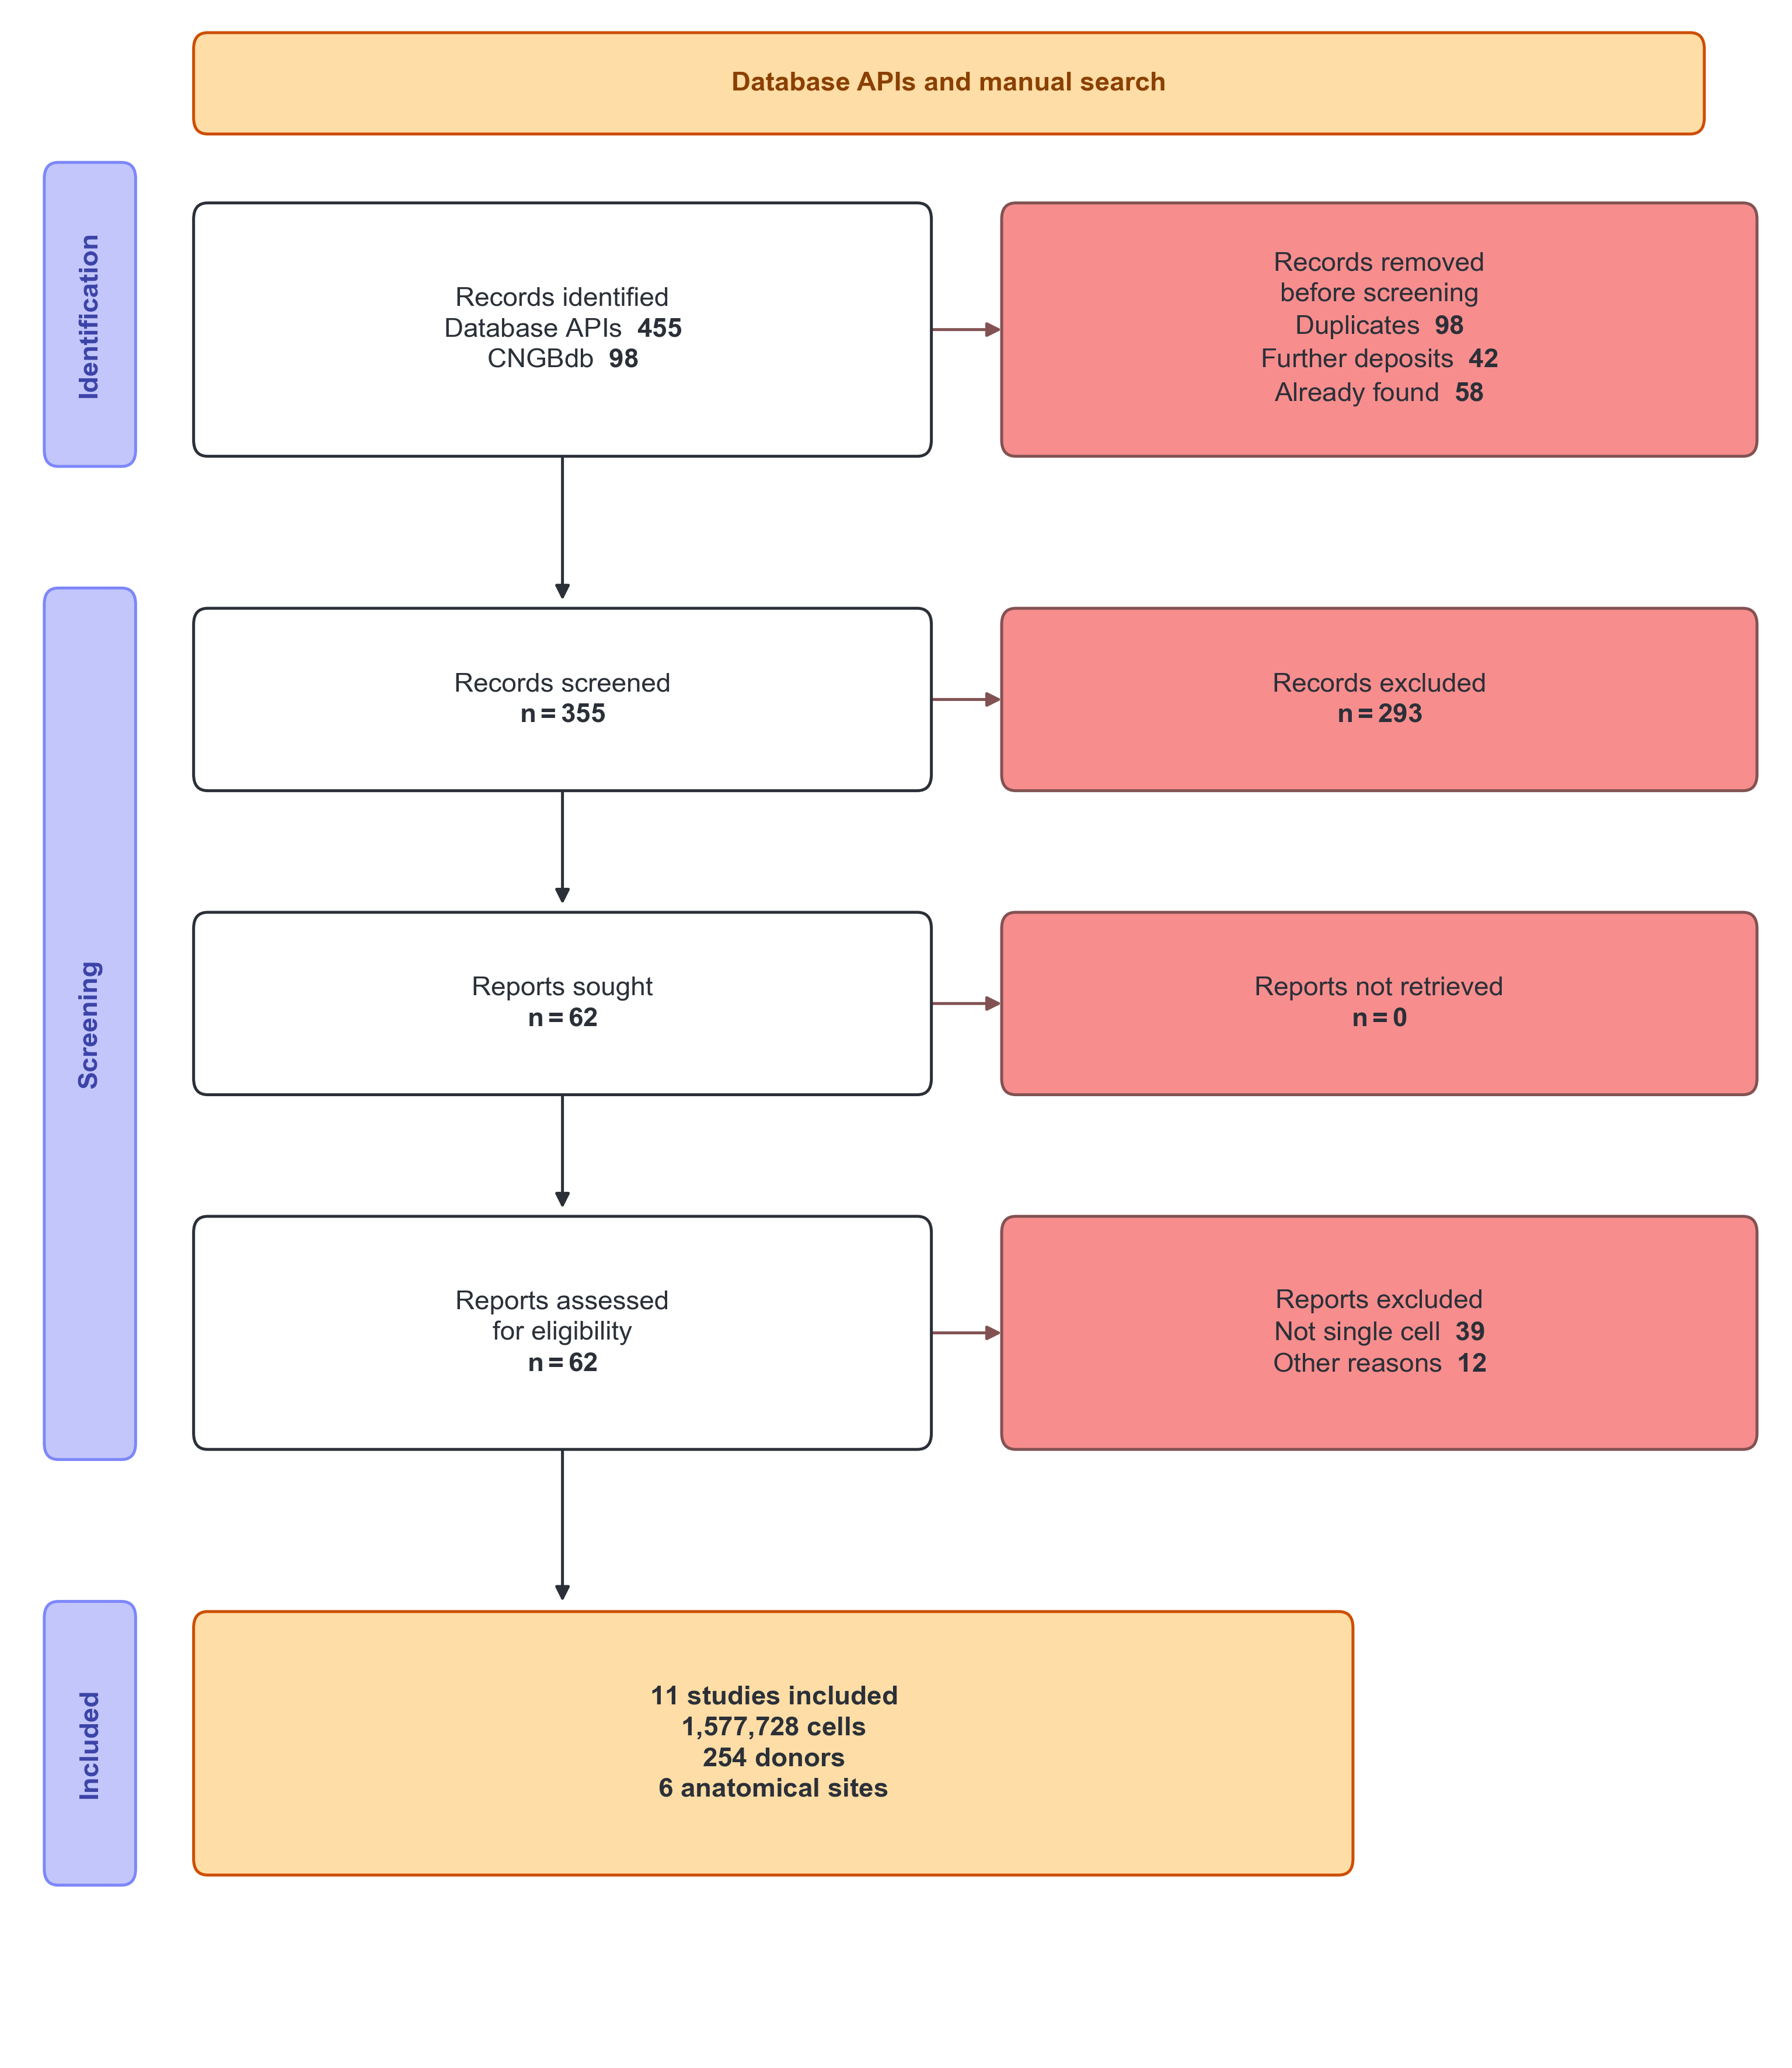
\includegraphics[width=0.72\linewidth]{figures/pinned/extdata1_prisma.png}
\caption{\textbf{Record selection, following PRISMA 2020.} The database and
manual routes are shown as one flow. Of 553 records identified, 198 were
removed before screening, 293 were excluded at screening and 51 of the 62
assessed were excluded, leaving 11 studies, 1{,}577{,}728 cells and 254 donors
across six anatomical sites. The arithmetic reconciles exactly: 455 records
from database APIs and 98 from CNGBdb, less 98 duplicates, 42 further deposits
and the 58 manual records the APIs had already returned, leaves 355 screened.}
\label{fig:prisma}
\end{figure}

\section*{Supplementary Information}
\note{Uncapped, and NMI's stated home for ``information not directly
related to the description of the main findings, but needed to properly
understand and replicate the study''. Things a reader consults rather
than reads:
\\$\bullet$ the accession table for all eleven studies;
\\$\bullet$ the gene vocabulary and how it was derived from Reactome and GO;
\\$\bullet$ the full reconstruction forward pass with every shape, and what
each of the six learned objects in the head uniquely holds, drawn from
docs/walkthrough/15-flow-reconstruction.md;
\\$\bullet$ the rank bound on the gene-query matrix, cut from Methods;
\\$\bullet$ the full factorial results and the seeds;
\\$\bullet$ every hyperparameter, per AW's ruling that configuration detail
goes to Code availability and Supplementary rather than into prose.}


% =====================================================================
%  REFERENCES
% =====================================================================
\bibliography{references}

\end{document}
